%%%%%%%%%%%%%%%%%%%%%%%%%%%%%%%%%%%%%%%%%%%%%%%%%%%%%%%%%%%%%%%%%%%%%%%%%%%%%%%

\documentclass[a4paper,10pt]{llncs}

%%%%%%%%%%%%%%%%%%%%%%%%%%%%%%%%%%%%%%%%%%%%%%%%%%%%%%%%%%%%%%%%%%%%%%%%%%%%%%%

\usepackage[utf8x]{inputenc}
\usepackage{amssymb}
\usepackage{amsmath}
\usepackage{amsfonts}
\usepackage{graphicx}
%\usepackage{llncsdoc}
\usepackage[english]{babel}
\usepackage[ruled,vlined,linesnumbered]{algorithm2e}
\usepackage{algorithmic}
\usepackage{float}
\usepackage{todonotes}
\usepackage{subfigure}
\usepackage{enumitem}
\usepackage{shuffle}

\usepackage{tikz}
\usetikzlibrary{matrix, calc, arrows, shapes.callouts}

%%%%%%%%%%%%%%%%%%%%%%%%%%%%%%%%%%%%%%%%%%%%%%%%%%%%%%%%%%%%%%%%%%%%%%%%%%%%%%%

%%% 
%%% complexity.tex
%%% 

\usepackage{xspace}

%%% ----------------------------------------------------------------------
%%% complexity classes
%%% ----------------------------------------------------------------------

% TIME
\newcommand{\DTIMEX}{{\sf\bf DTIME}}
\newcommand{\DTIMEclass}{\DTIMEX\xspace}
\newcommand{\DTIME}{\DTIMEclass}
% NL class
\newcommand{\NLclassbase}{{\sf\bf NL}}
\newcommand{\NLclass}{\NLclassbase\xspace}
% P class
\newcommand{\Pclassbase}{{\sf\bf P}}
\newcommand{\Pclass}{\Pclassbase\xspace}
% NP class
\newcommand{\NPclassbase}{{\sf\bf NP}}
\newcommand{\NPclass}{\NPclassbase\xspace}
% coNP class
\newcommand{\coNPclassbase}{{\sf\bf coNP}}
\newcommand{\coNPclass}{\coNPclassbase\xspace}
% PSPACE class
\newcommand{\PSPACEclassbase}{{\sf\bf PSPACE}}
\newcommand{\PSPACEclass}{\PSPACEclassbase\xspace}
% MAXSNP class
\newcommand{\MaxSNPclassbase}{{\sf\bf MaxSNP}}
\newcommand{\MaxSNPclass}{\MaxSNPclassbase\xspace}
% MAXNP class
\newcommand{\MaxNPclassbase}{{\sf\bf MaxNP}}
\newcommand{\MaxNPclass}{\MaxNPclassbase\xspace}
% EPTAS class
\newcommand{\EPTASclassbase}{{\sf\bf EPTAS}}
\newcommand{\EPTASclass}{\EPTASclassbase\xspace}
% FPTAS class
\newcommand{\FPTASclassbase}{{\sf\bf FPTAS}}
\newcommand{\FPTASclass}{\FPTASclassbase\xspace}
% PTAS class
\newcommand{\PTASclassbase}{{\sf\bf PTAS}}
\newcommand{\PTASclass}{\PTASclassbase\xspace}
% APX class
\newcommand{\APXclassbase}{{\sf\bf APX}}
\newcommand{\APXclass}{\APXclassbase\xspace}
% log-APX class
\newcommand{\logAPXclassbase}{{\sf\bf log{\tt -}APX}}
\newcommand{\logAPXclass}{\logAPXclassbase\xspace}
% poly-APX class
\newcommand{\polyAPXclassbase}{{\sf\bf poly{\tt -}APX}}
\newcommand{\polyAPXclass}{\polyAPXclassbase\xspace}
% exp-APX class
\newcommand{\expAPXclassbase}{{\sf\bf exp{\tt -}APX}}
\newcommand{\expAPXclass}{\expAPXclassbase\xspace}
% NPO class
\newcommand{\NPOclassbase}{{\sf\bf NPO}}
\newcommand{\NPOclass}{\NPOclassbase\xspace}
% #P class
\newcommand{\sharpPclassbase}{\#{\sf\bf P}}
\newcommand{\sharpPclass}{\sharpPclassbase\xspace}
% FPT class
\newcommand{\FPTclassbase}{{\sf\bf FPT}}
\newcommand{\FPTclass}{\FPTclassbase\xspace}
% W class
\newcommand{\Wclassbase}[1]{{\sf\bf W[#1]}}
\newcommand{\Wclass}[1]{\Wclassbase{#1}\xspace}
% W class
\newcommand{\XPclassbase}{{\sf\bf XP}}
\newcommand{\XPclass}{\XPclassbase\xspace}
% WNL class
\newcommand{\WNLclassbase}{{\sf\bf WNL}}
\newcommand{\WNLclass}{\WNLclassbase\xspace}
% ZPP class
\newcommand{\ZPPclassbase}{{\sf\bf ZPP}}
\newcommand{\ZPPclass}{\ZPPclassbase\xspace}
% NPK class
\newcommand{\NPKclassbase}{{\sf\bf NPK}}
\newcommand{\NPKclass}{\NPKclassbase\xspace}
\newcommand{\NPKandclass}{\text{$\NPKclass_\text{and}$}\xspace}
\newcommand{\NPKzeroandclass}{\text{$\NPKclass^0_\text{and}$}\xspace}
\newcommand{\NPKorclass}{\text{$\NPKclass_\text{or}$}\xspace}
\newcommand{\NPKzeroorclass}{\text{$\NPKclass^0_\text{or}$}\xspace}

%%% ----------------------------------------------------------------------
%%% complete
%%% ----------------------------------------------------------------------

% keyword
\newcommand{\complete}{\text{-complete}}
% NL-complete
\newcommand{\NLcomplete}{\NLclassbase\complete\xspace}
\newcommand{\NLC}{\NLcomplete}
% P-complete
\newcommand{\Pcomplete}{\Pclassbase\complete\xspace}
\newcommand{\PC}{\Pcomplete}
% NP-complete
\newcommand{\NPcomplete}{\NPclassbase\complete\xspace}
\newcommand{\NPC}{\NPcomplete}
% coNP-complete
\newcommand{\coNPcomplete}{\coNPclassbase\complete\xspace}
\newcommand{\coNPC}{\coNPcomplete}
% PSPACE-complete
\newcommand{\PSPACEcomplete}{\PSPACEclassbase\complete\xspace}
\newcommand{\PSPACEC}{\PSPACEcomplete}
% MAXSNP-complete
\newcommand{\MaxSNPcomplete}{\MaxSNPclassbase\complete\xspace}
\newcommand{\MaxSNPC}{\MaxSNPcomplete}
% APX-complete
\newcommand{\APXcomplete}{\APXclassbase\complete\xspace}
\newcommand{\APXC}{\APXcomplete}
% #P-complete
\newcommand{\sharpPcomplete}{\sharpPclassbase\complete\xspace}
\newcommand{\sharpPC}{\sharpPcomplete}
% W[i]-complete
\newcommand{\Wcomplete}[1]{\Wclassbase{#1}\complete\xspace}
\newcommand{\WC}[1]{\Wcomplete{#1}}
% WNL-complete
\newcommand{\WNLcomplete}{\WNLclassbase\complete\xspace}
\newcommand{\WNLC}{\WNLcomplete}

%%% ----------------------------------------------------------------------
%%% hard
%%% ----------------------------------------------------------------------

% keyword
\newcommand{\hard}{\text{-hard}}
% NL-hard
\newcommand{\NLhard}{\NLclassbase\hard\xspace}
\newcommand{\NLH}{\NLhard}
% P-hard
\newcommand{\Phard}{\NPclassbase\hard\xspace}
\newcommand{\PH}{\Phard}
% NP-hard
\newcommand{\NPhard}{\NPclassbase\hard\xspace}
\newcommand{\NPH}{\NPhard}
% coNP-hard
\newcommand{\coNPhard}{\coNPclassbase\hard\xspace}
\newcommand{\coNPH}{\coNPhard}
% PSPACE-hard
\newcommand{\PSPACEhard}{\PSPACEclassbase\hard\xspace}
\newcommand{\PSPACEH}{\PSPACEhard}
% MAXSNP-hard
\newcommand{\MaxSNPhard}{\MaxSNPclassbase\hard\xspace}
\newcommand{\MaxSNPH}{\MaxSNPhard}
% APX-hard
\newcommand{\APXhard}{\APXclassbase\hard\xspace}
\newcommand{\APXH}{\APXhard}
% WNL-hard
\newcommand{\WNLhard}{\WNLclassbase\hard\xspace}
\newcommand{\WNLH}{\WNLhard}
% #P-hard
\newcommand{\sharpPhard}{\sharpPclassbase\hard\xspace}
\newcommand{\sharpPH}{\sharpPhard}
% W[i]-hard
\newcommand{\Whard}[1]{\Wclassbase{#1}\hard\xspace}
\newcommand{\WH}[1]{\Whard{#1}}

%%% ----------------------------------------------------------------------
%%% hardness
%%% ----------------------------------------------------------------------

% keyword
\newcommand{\hardness}{\text{-hardness}}
% NP-hardness
\newcommand{\NPhardness}{\NPclassbase\hardness\xspace}
% APX-hardness
\newcommand{\APXhardness}{\APXclassbase\hardness\xspace}
% W[i]-hardness
\newcommand{\Whardness}[1]{\Wclassbase{#1}\hardness\xspace}
% WNL-hardness
\newcommand{\WNLhardness}{\WNLclassbase\hardness\xspace}

%%% ----------------------------------------------------------------------
%%% completeness
%%% ----------------------------------------------------------------------

% keyword
\newcommand{\completeness}{\text{-completeness}}
% NL-completeness
\newcommand{\NLcompleteness}{\NLclassbase\completeness\xspace}
% P-completeness
\newcommand{\Pcompleteness}{\NPclassbase\completeness\xspace}
% NP-completeness
\newcommand{\NPcompleteness}{\NPclassbase\completeness\xspace}
% APX-completeness
\newcommand{\APXcompleteness}{\APXclassbase\completeness\xspace}
% #P-completeness
\newcommand{\sharpPcompleteness}{\sharpPclassbase\completeness\xspace}
% W[i]-hard
\newcommand{\Wcompleteness}[1]{\W{#1}-\completeness\xspace}

%%% ----------------------------------------------------------------------
%%% reduction
%%% ----------------------------------------------------------------------

\newcommand{\reduction}{reduction}
\newcommand{\reductions}{reductions}
\newcommand{\reductible}{reductible}

\newcommand{\APTypeReduction}{AP}
\newcommand{\PTASTypeReduction}{PTAS}
\newcommand{\LTypeReduction}{L}
\newcommand{\ETypeReduction}{E}
\newcommand{\fptTypeReduction}{fpt}
\newcommand{\pptTypeReduction}{ptp}

% AP-reduction
\newcommand{\APreduction}{\APTypeReduction-\reduction\xspace}
\newcommand{\APreductions}{\APTypeReduction-\reductions\xspace}
\newcommand{\APreductible}{\APTypeReduction-\reductible\xspace}

% PTAS-reduction
\newcommand{\PTASeduction}{\PTASTypeReduction-\reduction\xspace}
\newcommand{\PTASreductions}{\PTASTypeReduction-\reductions\xspace}
\newcommand{\PTASreductible}{\PTASTypeReduction-\reductible\xspace}

% L-reduction
\newcommand{\Lreduction}{\LTypeReduction-\reduction\xspace}
\newcommand{\Lreductions}{\LTypeReduction-\reductions\xspace}
\newcommand{\Lreductible}{\LTypeReduction-\reductible\xspace}

% E-reduction
\newcommand{\Ereduction}{\ETypeReduction-\reduction\xspace}
\newcommand{\Ereductions}{\ETypeReduction-\reductions\xspace}
\newcommand{\Ereductible}{\ETypeReduction-\reductible\xspace}

% fpt-reduction
\newcommand{\fptreduction}{\fptTypeReduction-\reduction\xspace}
\newcommand{\fptreductions}{\fptTypeReduction-\reductions\xspace}
\newcommand{\fptreductible}{\fptTypeReduction-\reductible\xspace}

% ptp-reduction
\newcommand{\ptpreduction}{\ptpTypeReduction-\reduction\xspace}
\newcommand{\ptpreductions}{\ptpTypeReduction-\reductions\xspace}
\newcommand{\ptpreductible}{\ptpTypeReduction-\reductible\xspace}

% symbols
\DeclareMathOperator{\APreduce}{\text{$\leq_{\text{\APTypeReduction}}$}}
\DeclareMathOperator{\PTASreduce}{\text{$\leq_{\text{\PTASTypeReduction}}$}}
\DeclareMathOperator{\Lreduce}{\text{$\leq_{\text{\LTypeReduction}}$}}
\DeclareMathOperator{\Ereduce}{\text{$\leq_{\text{\ETypeReduction}}$}}
\DeclareMathOperator{\fptreduce}{\text{$\leq_{\text{\fptTypeReduction}}$}}
\DeclareMathOperator{\ptpreduce}{\text{$\leq_{\text{\fptTypeReduction}}$}}

%% 
%% Approximation
%%
\DeclareMathOperator{\poly}{poly}
\DeclareMathOperator{\POLY}{poly}
\DeclareMathOperator{\SIZE}{size}
\newcommand{\sol}{{\sf sol}\xspace}
\newcommand{\PB}[1]{\textsf{\scshape{#1}}}
\newcommand{\OPTname}{opt}
\newcommand{\OPT}{\text{$\mathsf{\bf \OPTname}$}}
\newcommand{\OPTpb}[1]{\text{$\mathsf{\OPTname}_{\PB{#1}}$}}
\newcommand{\ALGO}[1]{\textbf{\ttfamily\sf #1}}
\newcommand{\Approxname}{Approx}
\newcommand{\APPROX}[1]{\text{$\ALGO{\Approxname}_{\,\PB{#1}}$}}
\newcommand{\PCP}{{\sf\bf PCP}\xspace}

%%
%% Problem Definition
%%
\newcommand{\PbDef}[3]{%
\begin{center}
  \begin{tabular}{l}%
    \shadowbox{%
    \begin{minipage}[c]{.9\textwidth}
      \smallskip%
      \par\noindent%
      {#1}%
      \smallskip
      \par\noindent%
      $\bullet$
      \textbf{\textsf{Input}}~: #2% 
      \medskip
      \par\noindent%
      $\bullet$
      \textbf{\textsf{Question}}~:
      #3% 
      \smallskip%
      \par\noindent%
    \end{minipage}
  }% end shadowbox
  \end{tabular}%
\end{center}
}%
\newcommand{\PbDefinition}{\PbDef}

%%
%% Problem (Input + Output) Definition
%%
\newcommand{\PbInputOutputDef}[3]{%
\begin{center}
  \begin{tabular}{l}%
    \shadowbox{%
    \begin{minipage}[c]{.9\textwidth}
      \smallskip%
      \par\noindent%
      \PB{#1}%
      \medskip%
      \par\noindent%
      $\bullet$
      \textbf{\textsf{Input}}~: #2% 
      \medskip
      \par\noindent%
      $\bullet$
      \textbf{\textsf{Output}}~:
      #3% 
      \smallskip%
      \par\noindent%
    \end{minipage}
  }% end shadowbox
  \end{tabular}%
\end{center}
}%
\newcommand{\PbInputOutputDefinition}{\PbInputOutputDef}


%%
%% Optimization Problem Definition
%%

\newcommand{\OptPbDefinition}[4]{%
\begin{center}
  \begin{tabular}{l}%
    \shadowbox{%
    \begin{minipage}[c]{.9\textwidth}
      \par\noindent%
      \shadowbox{#1}%
      \par\noindent%
      $\bullet$
      \textbf{\textsf{Input}}~: #2% 
      \par\noindent%
      $\bullet$
      \textbf{\textsf{Solution}}~: #3%  
      \par\noindent%
      $\bullet$
      \textbf{\textsf{Measure}}~: #4% 
      \par\noindent%
    \end{minipage}
    }% end shadowbox
  \end{tabular}%
\end{center}
}%

%%
%% Parameterized Problem Definition
%%
\newcommand{\ParamPbDefinition}[4]{%
\begin{center}
  \begin{tabular}{l}%
    %\shadowbox{%
    \begin{minipage}[c]{.95\textwidth}
      % \smallskip%
      \par\noindent%
      #1%
      % \smallskip%
      \par\noindent%
      \textbf{\textsf{Input}}~: #2% 
      % \smallskip
      \par\noindent%
      \textbf{\textsf{Question}}~: #3%  
      % \smallskip
      \par\noindent%
      \textbf{\textsf{Parameter}}~: #4% 
      %\smallskip%
      \par\noindent%
    \end{minipage}
  %}% end shadowbox
  \end{tabular}%
\end{center}
}%
\newcommand{\ParamPbDefinitionTwo}[5]{%
\begin{center}
  \begin{tabular}{l}%
    \shadowbox{%
    \begin{minipage}[c]{.9\textwidth}
      \smallskip%
      \par\noindent%
      \shadowbox{#1}%
      \medskip%
      \par\noindent%
      $\bullet$
      \textbf{\textsf{Input}}~: #2% 
%      \medskip
      \par\noindent%
      $\bullet$
      \textbf{\textsf{Parameter}}~: #3% 
 %     \medskip
      \par\noindent%
      $\bullet$
      \textbf{\textsf{Parameter}}~: #4% 
      \medskip
      \par\noindent%
      $\bullet$
      \textbf{\textsf{Question}}~: #5%  
      \smallskip%
      \par\noindent%
    \end{minipage}
    }% end shadowbox
  \end{tabular}%
\end{center}
}%
\newcommand{\ParamPbDefinitionThree}[6]{%
\begin{center}
  \begin{tabular}{l}%
    \shadowbox{%
    \begin{minipage}[c]{.9\textwidth}
      \smallskip%
      \par\noindent%
      \shadowbox{#1}%
      \medskip%
      \par\noindent%
      $\bullet$
      \textbf{\textsf{Input}}~: #2% 
%      \medskip
      \par\noindent%
      $\bullet$
      \textbf{\textsf{Parameter}}~: #3% 
%      \medskip
      \par\noindent%
      $\bullet$
      \textbf{\textsf{Parameter}}~: #4% 
%      \medskip
      \par\noindent%
      $\bullet$
      \textbf{\textsf{Parameter}}~: #5%  
      \medskip
      \par\noindent%
      $\bullet$
      \textbf{\textsf{Question}}~: #6%  
      \smallskip%
      \par\noindent%
    \end{minipage}
    }% end shadowbox
  \end{tabular}%
\end{center}
}%
\newcommand{\ParamPbDefinitionFour}[7]{%
\begin{center}
  \begin{tabular}{l}%
    \shadowbox{%
    \begin{minipage}[c]{.9\textwidth}
      \smallskip%
      \par\noindent%
      \shadowbox{#1}%
      \medskip%
      \par\noindent%
      $\bullet$
      \textbf{\textsf{Input}}~: #2% 
%      \medskip
      \par\noindent%
      $\bullet$
      \textbf{\textsf{Parameter}}~: #3% 
%      \medskip
      \par\noindent%
      $\bullet$
      \textbf{\textsf{Parameter}}~: #4% 
%      \medskip
      \par\noindent%
      $\bullet$
      \textbf{\textsf{Parameter}}~: #5%  
%      \medskip
      \par\noindent%
    $\bullet$
      \textbf{\textsf{Parameter}}~: #6%  
      \medskip
      \par\noindent%
      $\bullet$
      \textbf{\textsf{Question}}~: #7%  
      \smallskip%
      \par\noindent%
    \end{minipage}
    }% end shadowbox
  \end{tabular}%
\end{center}
}%
\newcommand{\ParamPbDefinitionFive}[8]{%
\begin{center}
  \begin{tabular}{l}%
    \shadowbox{%
    \begin{minipage}[c]{.9\textwidth}
      \smallskip%
      \par\noindent%
      \shadowbox{#1}%
      \medskip%
      \par\noindent%
      $\bullet$
      \textbf{\textsf{Input}}~: #2% 
%      \medskip
      \par\noindent%
      $\bullet$
      \textbf{\textsf{Parameter}}~: #3% 
%      \medskip
      \par\noindent%
      $\bullet$
      \textbf{\textsf{Parameter}}~: #4% 
%      \medskip
      \par\noindent%
      $\bullet$
      \textbf{\textsf{Parameter}}~: #5%  
%      \medskip
      \par\noindent%
    $\bullet$
      \textbf{\textsf{Parameter}}~: #6%  
%      \medskip
      \par\noindent%
    $\bullet$
      \textbf{\textsf{Parameter}}~: #7%  
      \medskip
      \par\noindent%
      $\bullet$
      \textbf{\textsf{Question}}~: #8%  
      \smallskip%
      \par\noindent%
    \end{minipage}
    }% end shadowbox
  \end{tabular}%
\end{center}
}%
\newcommand{\ParamPbDefinitionSix}[9]{%
\begin{center}
  \begin{tabular}{l}%
    \shadowbox{%
    \begin{minipage}[c]{.9\textwidth}
      \smallskip%
      \par\noindent%
      \shadowbox{#1}%
      \medskip%
      \par\noindent%
      $\bullet$
      \textbf{\textsf{Input}}~: #2% 
%      \medskip
      \par\noindent%
      $\bullet$
      \textbf{\textsf{Parameter}}~: #3% 
%      \medskip
      \par\noindent%
      $\bullet$
      \textbf{\textsf{Parameter}}~: #4% 
%      \medskip
      \par\noindent%
      $\bullet$
      \textbf{\textsf{Parameter}}~: #5%  
%      \medskip
      \par\noindent%
      $\bullet$
      \textbf{\textsf{Parameter}}~: #6%  
%      \medskip
      \par\noindent%
      $\bullet$
      \textbf{\textsf{Parameter}}~: #7%  
%      \medskip
      \par\noindent%
      $\bullet$
      \textbf{\textsf{Parameter}}~: #8%  
      \medskip
      \par\noindent%
      $\bullet$
      \textbf{\textsf{Question}}~: #9%  
      \smallskip%
      \par\noindent%
    \end{minipage}
    }% end shadowbox
  \end{tabular}%
\end{center}
}%




%%%%%%%%%%%%%%%%%%%%%%%%%%%%%%%%%%%%%%%%%%%%%%%%%%%%%%%%%%%%%%%%%%%%%%%%%%%%%%%

% \renewcommand{\floatpagefraction}{.9}
% \renewcommand{\textfraction}{.1}

%%%%%%%%%%%%%%%%%%%%%%%%%%%%%%%%%%%%%%%%%%%%%%%%%%%%%%%%%%%%%%%%%%%%%%%%%%%%%%%

\DeclareMathOperator{\LEFT}{\ell}
\DeclareMathOperator{\RIGHT}{r}
\DeclareMathOperator{\QQ}{\mathbb{Q}}
\DeclareMathOperator{\STD}{\mathrm{s}}
\DeclareMathOperator{\SHUFFLE}{\bullet}
\DeclareMathOperator{\BINTOPERM}{\mathrm{btp}}
\DeclareMathOperator{\PERMTOBIN}{\mathrm{ptb}}

%%%%%%%%%%%%%%%%%%%%%%%%%%%%%%%%%%%%%%%%%%%%%%%%%%%%%%%%%%%%%%%%%%%%%%%%%%%%%%%

\newtheorem{fact}{Fact}

%%%%%%%%%%%%%%%%%%%%%%%%%%%%%%%%%%%%%%%%%%%%%%%%%%%%%%%%%%%%%%%%%%%%%%%%%%%%%%%

\makeatletter
\newcommand{\pushright}[1]{\ifmeasuring@#1\else\omit\hfill$\displaystyle#1$\fi\ignorespaces}
\newcommand{\pushleft}[1]{\ifmeasuring@#1\else\omit$\displaystyle#1$\hfill\fi\ignorespaces}
\makeatother

%%%%%%%%%%%%%%%%%%%%%%%%%%%%%%%%%%%%%%%%%%%%%%%%%%%%%%%%%%%%%%%%%%%%%%%%%%%%%%%

\begin{document}

%%%%%%%%%%%%%%%%%%%%%%%%%%%%%%%%%%%%%%%%%%%%%%%%%%%%%%%%%%%%%%%%%%%%%%%%%%%%%%%

\title{%
Unshuffling Permutations}%

\author{%
  Samuele Giraudo \and
  St\'ephane Vialette
}% end author
\institute{%
  Universit\'e Paris-Est, LIGM (UMR 8049), CNRS, UPEM, ESIEE Paris, ENPC,
  F-77454, Marne-la-Vallée, France\\
  \email{samuele.giraudo@univ-mlv.fr} \\
  \email{vialette@univ-mlv.fr}
}% end institute
\date{\today}

\maketitle

%%%%%%%%%%%%%%%%%%%%%%%%%%%%%%%%%%%%%%%%%%%%%%%%%%%%%%%%%%%%%%%%%%%%%%%%%%%%%%%

\begin{abstract}
bla bla bla \ldots
\end{abstract}

%%%%%%%%%%%%%%%%%%%%%%%%%%%%%%%%%%%%%%%%%%%%%%%%%%%%%%%%%%%%%%%%%%%%%%%%%%%%%%%

%%
%%
%% ---- Introduction ----
%%
\section{Introduction}
\label{section:Introduction}


%%%%%%%%%%%%%%%%%%%%%%%%%%%%%%%%%%%%%%%%%%%%%%%%%%%%%%%%%%%%%%%%%%%%%%%%%%%%%%%

%%
%% ---- Notations ----
%%
\section{Notations}
\label{section:Notations}

We denote by $S_n$ the set of permutations of size $n$ and by $S$ the
set of all permutations. If $\pi$ is a permutation, we denote by $|\pi|$
its size. The unique permutation of size $0$ is denoted by $\epsilon$.
If $P$ is a subset of $[|\pi|]$, $\pi_{|P}$ is the subword of $\pi$
consisting in the letters of $\pi$ at the positions specified by the
elements of $P$. Besides, we denote by $\widetilde{\pi}$ (resp.
$\bar \pi$, $\pi^{-1}$) the mirror image (resp. complementary, inverse)
of $\pi$. If $u$ is a word of integers without multiple occurrences of a
same letter, $\STD(u)$ denotes the unique permutation of same size as
$u$ such that for all $i, j \in [|u|]$, $u_i < u_j$ if and only if
$\STD(u)_i < \STD(u)_j$.
\medskip

%%%%%%%%%%%%%%%%%%%%%%%%%%%%%%%%%%%%%%%%%%%%%%%%%%%%%%%%%%%%%%%%%%%%%%%%%%%%%%%

%%
%% ---- Algebraic issues ----
%%
\section{Algebraic issues}
\label{section:Algebraic issues}
The purpose of this section is to define a shuffle product $\SHUFFLE$
on permutations and establish some of its properties. To define this
shuffle product, we shall first define a coproduct denoted by $\Delta$.
By duality, $\Delta$ implies the definition of $\SHUFFLE$. It is worth
to note that, as we will see, algebraic properties of $\Delta$ imply
combinatorial properties of $\SHUFFLE$. We invite the reader unfamiliar
with the concepts of coproduct and duality to consult~\cite{Joni:Rota:1979}
or~\cite{Grinberg:Reiner:2014}.
\medskip

Let use denote by $\QQ[S]$ the linear span of all permutations. As
announced, we shall define on this space a kind of shuffle product and
for this purpose, we first define a linear coproduct $\Delta$ on $\QQ[S]$.
For any permutation $\pi$, we set
\begin{equation} \label{equ:unshuffling_coproduct}
    \Delta(\pi) =
    \sum_{P_1 \uplus P_2 = [|\pi|]}
    \STD\left(\pi_{|P_1}\right) \otimes \STD\left(\pi_{|P_2}\right).
\end{equation}
We call $\Delta$ the {\em unshuffling coproduct of permutations}. For
instance,
\begin{equation}
    \Delta(213) =
    \epsilon \otimes 213 + 2. 1 \otimes 12 +
    1 \otimes 21 + 2. 12 \otimes 1 + 21 \otimes 1 + 213 \otimes \epsilon,
\end{equation}
\begin{equation}
    \Delta(1234) =
    \epsilon \otimes 1234 + 4. 1 \otimes 123 + 6. 12 \otimes 12 +
    4. 123 \otimes 1 + 1234 \otimes \epsilon,
\end{equation}
\begin{equation}\begin{split} \label{equ:example_unshuffling_coproduct}
    \Delta(1432) & =
    \epsilon \otimes 1432 + 3. {\bf 1 \otimes 132} + 1 \otimes 321 +
    3. 12 \otimes 21 \\ & + 3. 21 \otimes 12 + 3. 132 \otimes 1 +
    321 \otimes 1 + 1432 \otimes \epsilon.
\end{split}\end{equation}
Observe that the coefficient of the tensor $1 \otimes 132$ is $3$
in~\eqref{equ:example_unshuffling_coproduct} because there are exactly
three ways to extract two disjoint subwords of the permutation $1432$
so that the letters of these two subwords have respectively the same
relative order as the letters of the permutations $1$ and $132$.
\medskip

As any coproduct, $\Delta$ leads to the definition of a product obtained
by duality in the following way. From~\eqref{equ:unshuffling_coproduct},
for any permutation $\pi$, we have
\begin{equation} \label{equ:schematic_coproduct}
    \Delta(\pi) =
    \sum_{\sigma, \nu \in S} \lambda_{\sigma, \nu}^\pi \;
    \sigma \otimes \nu,
\end{equation}
where the $\lambda_{\sigma, \nu}^\pi$ are nonnegative integers. Now,
by definition of duality, the dual product of $\Delta$ denoted by
$\SHUFFLE$ is a linear binary product on $\QQ[S]$. It satisfies, for any
permutations
$\sigma$ and $\nu$,
\begin{equation}
    \sigma \SHUFFLE \nu =
    \sum_{\pi \in S}
    \lambda_{\sigma, \nu}^\pi \; \pi,
\end{equation}
where the coefficients $\lambda_{\sigma, \nu}^\pi$ are the ones
of~\eqref{equ:schematic_coproduct}. We call $\SHUFFLE$ the
{\em shuffle product of permutations}. For instance,
\begin{equation}\begin{split} \label{equ:example_shuffle_product}
    12 \SHUFFLE 21 & =
    1243 + 1324 + 2.1342 + 2.1423 + 3. {\bf 1432} + 2134 + 2.2314 \\
    & + 3.2341 + 2413 + 2.2431 + 2.3124 + 3142 + 3.3214 + 2.3241 \\
    & + 3421 + 3.4123 + 2.4132 + 2.4213 + 4231 + 4312.
\end{split}\end{equation}
Observe that the coefficient $3$ of the permutation $1432$
in~\eqref{equ:example_shuffle_product} comes from the fact that the
coefficient of the tensor $12 \otimes 21$ is $3$
in~\eqref{equ:example_unshuffling_coproduct}.
\medskip

Intuitively, this product shuffles the values and the positions of the
letters of the permutations. There are other shuffle products on
permutations~\cite{DHT:IJAC:2002}: the {\em shifted shuffle} and the
{\em convolution product}. Our shuffle product is different from these
last two.
\medskip

We say that a permutation $\pi$ {\em appears} in the shuffle
$\sigma \SHUFFLE \nu$ of two permutations $\sigma$ and $\nu$ if the
coefficient $\lambda_{\sigma, \nu}^\pi$ defined aboev is different from
zero. Besides, a permutation $\pi$ is a {\em square} if there is a
permutation $\sigma$ such that $\pi$ appears in $\sigma \SHUFFLE \sigma$.
In this case, we say that $\sigma$ is a {\em square root} of $\pi$.
Equivalently, $\pi$ is a square with $\sigma$ as square root if and only
if in the expansion of $\Delta(\pi)$, there is a tensor
$\sigma \otimes \sigma$ with a nonzero coefficient.
\medskip

\begin{proposition} \label{prop:shuffle_associative_commutative}
    The shuffle product $\SHUFFLE$ of permutations is associative and
    commutative.
\end{proposition}
\begin{proof}
    To prove the associativity of $\SHUFFLE$, it is convenient to show
    that its dual coproduct $\Delta$ is coassociative, that is
    \begin{equation}
        (\Delta \otimes I) \Delta = (I \otimes \Delta) \Delta,
    \end{equation}
    where $I$ denote the identity map. This strategy relies on the fact
    that a product is associative if and only if its dual coproduct is
    coassociative. For any permutation $\pi$, we have
    \begin{equation} \begin{split}
    \label{equ:shuffle_associative_commutative}
        (\Delta \otimes I) \Delta(\pi) & =
        (\Delta \otimes I)
        \sum_{P_1 \uplus P_2 = [|\pi|]}
        \STD\left(\pi_{|P_1}\right) \otimes \STD\left(\pi_{|P_2}\right) \\
        & =
        \sum_{P_1 \uplus P_2 = [|\pi|]}
        \Delta\left(\STD\left(\pi_{|P_1}\right)\right)
        \otimes I\left(\STD\left(\pi_{|P_2}\right)\right) \\
        & =
        \sum_{P_1 \uplus P_2 = [|\pi|]} \;
        \sum_{Q_1 \uplus Q_2 = [|P_1|]}
        \STD\left(\STD\left(\pi_{|P_1}\right)_{|Q_1}\right)
        \otimes
        \STD\left(\STD\left(\pi_{|P_1}\right)_{|Q_2}\right)
        \otimes \STD\left(\pi_{|P_2}\right) \\
        & =
        \sum_{P_1 \uplus P_2 \uplus P_3 = [|\pi|]}
        \STD\left(\pi_{|P_1}\right) \otimes
        \STD\left(\pi_{|P_2}\right) \otimes
        \STD\left(\pi_{|P_3}\right).
    \end{split} \end{equation}
    An analogous computation shows that $(I \otimes \Delta) \Delta(\pi)$
    is equal to the last member
    of~\eqref{equ:shuffle_associative_commutative}, whence the
    associativity of $\SHUFFLE$.
    \smallskip

    Finally, to prove the commutativity of $\SHUFFLE$, we shall show
    that $\Delta$ is cocommutative, that is for any permutation $\pi$,
    if in the expansion of $\Delta(\pi)$ there is a tensor
    $\sigma \otimes \nu$ with a coefficient $\lambda$, there is in the
    same expansion the tensor $\nu \otimes \sigma$ with the same
    coefficient $\lambda$. Clearly, a product is commutative if and only
    if its dual coproduct is cocommutative. Now, from the
    definition~\eqref{equ:unshuffling_coproduct} of $\Delta$, one
    observes that if the pair $(P_1, P_2)$ of subsets of $[|\pi|]$
    contributes to the coefficient of
    $\STD\left(\pi_{|P_1}\right) \otimes \STD\left(\pi_{|P_2}\right)$,
    the pair $(P_2, P_1)$ contributes to the coefficient of
    $\STD\left(\pi_{|P_2}\right) \otimes \STD\left(\pi_{|P_1}\right)$.
    This shows that $\Delta$ is cocommutative and hence, that $\SHUFFLE$
    is commutative.
    \qed
\end{proof}
\medskip

Proposition~\ref{prop:shuffle_associative_commutative} implies that
$\QQ[S]$ endowed with the unshuffling coproduct $\Delta$ is a
coassociative cocommutative coalgebra, or in an equivalent way, that
$\QQ[S]$ endowed with the shuffle product $\SHUFFLE$ is an associative
commutative algebra.
\medskip

\begin{proposition} \label{prop:endomorphisms}
    The three linear maps
    \begin{equation}
        \phi_1, \phi_2, \phi_3 : \QQ[S] \to \QQ[S]
    \end{equation}
    linearly sending a permutation $\pi$ to, respectively,
    $\widetilde{\pi}$, $\bar \pi$, and $\pi^{-1}$ are endomorphims of
    associative algebras.
\end{proposition}
\begin{proof}
    To prove, for $j = 1, 2, 3$, that $\phi_j$ is a morphism of
    associative algebras, we have to prove that for all permutations
    $\sigma$ and $\nu$,
    \begin{equation}
        \phi_j(\sigma \SHUFFLE \nu) =
        \phi_j(\sigma) \SHUFFLE \phi_j(\nu).
    \end{equation}
    We shall proceed here as we have done during the proof of
    Proposition~\ref{prop:shuffle_associative_commutative} by showing
    that $\phi_j$ is a morphism of coalgebras, that is
    \begin{equation}
        \Delta \phi_j = (\phi_j \otimes \phi_j) \Delta.
    \end{equation}
    In the sequel, $\pi$ is a permutation.
    \smallskip

    If $P$ is a set of indexes of letters of $\pi$, we denote by
    $\widetilde{P}$ the set $\{|\pi| - i  + 1 : i \in P\}$. Now, since
    the operation $\widetilde{\,}$ define a bijection on the set of the
    subsets of $[|\pi|]$, and since the standardization operation
    commutes with the mirror operation on words, we have
    \begin{equation} \begin{split}
        \Delta(\phi_1(\pi))
        & = \sum_{P_1 \uplus P_2 = [|\pi|]}
        \STD\left(\phi_1(\pi)_{|P_1}\right)
        \otimes \STD\left(\phi_1(\pi)_{|P_2}\right) \\
        & = \sum_{P_1 \uplus P_2 = [|\pi|]}
        \STD\left(\widetilde{\pi}_{|P_1}\right)
        \otimes \STD\left(\widetilde{\pi}_{|P_2}\right) \\
        & = \sum_{P_1 \uplus P_2 = [|\pi|]}
        \STD\left(\widetilde{\pi}_{|\widetilde{P_1}}\right)
        \otimes \STD\left(\widetilde{\pi}_{|\widetilde{P_2}}\right) \\
        & = \sum_{P_1 \uplus P_2 = [|\pi|]}
        \widetilde{\STD\left(\pi_{|P_1}\right)}
        \otimes \widetilde{\STD\left(\pi_{|P_2}\right)} \\
        & = \sum_{P_1 \uplus P_2 = [|\pi|]}
        \phi_1\left(\STD\left(\pi_{|P_1}\right)\right)
        \otimes \phi_1\left(\STD\left(\pi_{|P_2}\right)\right) \\
        & = (\phi_1 \otimes \phi_1) \Delta(\pi).
    \end{split} \end{equation}
    This shows that $\phi_1$ is a morphism of coalgebras and hence, that
    $\phi_1$ is a morphism of associative algebras.
    \smallskip

    Next, since by definition of the complementation operation on
    permutations, for any permutation $\tau$ and any indexes $i$ and $k$,
    we have $\tau_i < \tau_k$ if and only if $\bar \tau_i > \bar \tau_k$,
    we have
    \begin{equation} \begin{split}
        \Delta(\phi_2(\pi))
        & = \sum_{P_1 \uplus P_2 = [|\pi|]}
        \STD\left(\phi_2(\pi)_{|P_1}\right)
        \otimes \STD\left(\phi_2(\pi)_{|P_2}\right) \\
        & = \sum_{P_1 \uplus P_2 = [|\pi|]}
        \STD\left(\bar \pi_{|P_1}\right)
        \otimes \STD\left(\bar \pi_{|P_2}\right) \\
        & = \sum_{P_1 \uplus P_2 = [|\pi|]}
        \phi_2\left(\STD\left(\pi_{|P_1}\right)\right)
        \otimes \phi_2\left(\STD\left(\pi_{|P_2}\right)\right) \\
        & = (\phi_2 \otimes \phi_2) \Delta(\pi).
    \end{split} \end{equation}
    This shows that $\phi_2$ is a morphism of coalgebras and hence, that
    $\phi_2$ is a morphism of associative algebras.
    \smallskip

    Finally, for any permutation $\tau$, if $P$ is a set of indexes of
    letters of $\tau$, we denote by $P_\tau^{-1}$ the set
    $\{\tau_i : i \in P\}$. Since the map sending a subset $P$ of
    $[|\pi|]$ to $P_\pi^{-1}$ is a bijection, and since
    $\STD\left(\pi_{|P}\right)^{-1} = \STD\left(\pi^{-1}_{|P_\pi^{-1}}\right)$,
    we have
    \begin{equation} \begin{split}
        \Delta(\phi_3(\pi))
        & = \sum_{P_1 \uplus P_2 = [|\pi|]}
        \STD\left(\phi_3(\pi)_{|P_1}\right)
        \otimes \STD\left(\phi_3(\pi)_{|P_2}\right) \\
        & = \sum_{P_1 \uplus P_2 = [|\pi|]}
        \STD\left(\pi^{-1}_{|P_1}\right)
        \otimes \STD\left(\pi^{-1}_{|P_2}\right) \\
        & = \sum_{P_1 \uplus P_2 = [|\pi|]}
        \STD\left(\pi^{-1}_{|{P_1}_\pi^{-1}}\right)
        \otimes \STD\left(\pi^{-1}_{|{P_2}_\pi^{-1}}\right) \\
        & = \sum_{P_1 \uplus P_2 = [|\pi|]}
        \STD\left(\pi_{|P_1}\right)^{-1}
        \otimes \STD\left(\pi_{|P_2}\right)^{-1} \\
        & = \sum_{P_1 \uplus P_2 = [|\pi|]}
        \phi_3\left(\STD\left(\pi_{|P_1}\right)\right)
        \otimes \phi_3\left(\STD\left(\pi_{|P_2}\right)\right) \\
        & = (\phi_3 \otimes \phi_3) \Delta(\pi).
    \end{split} \end{equation}
    This shows that $\phi_3$ is a morphism of coalgebras and hence, that
    $\phi_3$ is a morphism of associative algebras.
    \qed
\end{proof}
\medskip

We now use the algebraic properties of $\SHUFFLE$ exhibited by
Proposition~\ref{prop:endomorphisms} to obtain combinatorial properties
of square permutations.
\medskip

\begin{proposition} \label{prop:square_stability}
    Let $\pi$ be a square permutation and $\rho$ be a square root of
    $\pi$. Then,
    \begin{enumerate}[label={\it (\roman*)},fullwidth]
        \item \label{item:square_stability_1}
        the permutation $\widetilde{\pi}$ is a square and
        $\widetilde{\rho}$ is one of its square roots;
        \item \label{item:square_stability_2}
        the permutation $\bar \pi$ is a square and $\bar \rho$ is one of
        its square roots;
        \item \label{item:square_stability_3}
        the permutation $\pi^{-1}$ is a square and $\rho^{-1}$ is one of
        its square roots.
    \end{enumerate}
\end{proposition}
\begin{proof}
    All statements~\ref{item:square_stability_1},
    \ref{item:square_stability_2}, and~\ref{item:square_stability_3} are
    direct consequences of Proposition~\ref{prop:endomorphisms}. Indeed,
    since $\pi$ is a square permutation and $\rho$ is a square root of
    $\pi$, by definition, $\pi$ appears in the product
    $\rho \SHUFFLE \rho$. Now, by Proposition~\ref{prop:endomorphisms},
    for any $j = 1, 2, 3$, since $\phi_j$ is a morphism of associative
    algebras from $\QQ[S]$ to $\QQ[S]$, $\phi_j$ commutes with the
    shuffle product of permutations $\SHUFFLE$. Hence, in particular,
    one has
    \begin{equation}
        \phi_j(\rho \SHUFFLE \rho) =
        \phi_j(\rho) \SHUFFLE \phi_j(\rho).
    \end{equation}
    Then, since $\pi$ appears in $\rho \SHUFFLE \rho$, $\phi_j(\pi)$
    appears in $\phi_j(\rho \SHUFFLE \rho)$ and also in
    $\phi_j(\rho) \SHUFFLE \phi_j(\rho)$. This shows that
    $\phi_j(\rho)$ is a square root of $\phi_j(\pi)$ and
    implies~\ref{item:square_stability_1}, \ref{item:square_stability_2},
    and~\ref{item:square_stability_3}.
    \qed
\end{proof}
\medskip

%%%%%%%%%%%%%%%%%%%%%%%%%%%%%%%%%%%%%%%%%%%%%%%%%%%%%%%%%%%%%%%%%%%%%%%%%%%%%%%

%%
%% ---- Algorithmic issues ----
%%
\section{Algorithmic issues}
\label{section:Algorithmic issues}


\begin{proposition}
<<<<<<< HEAD
  \label{proposition:matching}
  Let $\pi \in S_{2n}$.
  Then,
  $\pi$ is the union of two order-isomorphic patterns
  if and only if
  there exists a perfect containment-free mathing
  $\mathcal{M}$ of $G_\pi$ such that
  $\LEFT(\mathcal{M}) \simeq \RIGHT(\mathcal{M})$.
=======
Let $\pi \in S_{2n}$.
Then,
$\pi$ is the union of two order-isomorphic pattern
if and only if
there exists a perfect containment-free mathing
$\mathcal{M}$ of $G_\pi$ such that
$\LEFT(\mathcal{M}) \simeq \RIGHT(\mathcal{M})$.
>>>>>>> 52a537603cf201d0e9be15f2ee3234f7c21d0df7
\end{proposition}

\begin{proposition}
  \label{proposition:hardness}
  Deciding whether a permutation is the union of two
  order-isomorphic patterns is \NPC.
\end{proposition}

\begin{proof}
  For the sake of clarity, we will that a bunch of positions $P$
  is \emph{above} (resp. \emph{below}) above another bunch of positions $P'$
  in permutation $\mu$
  if $\mu(x) > \mu(y)$ (resp. $\mu(x) < \mu(y)$) for every $x \in P$
  and every $y \in P'$.
  For exemple, $\nu_1$ is above $\nu_2$ but below $\nu'_1$ in permutation $\mu$.

  \begin{figure}[t!]
    \centering
    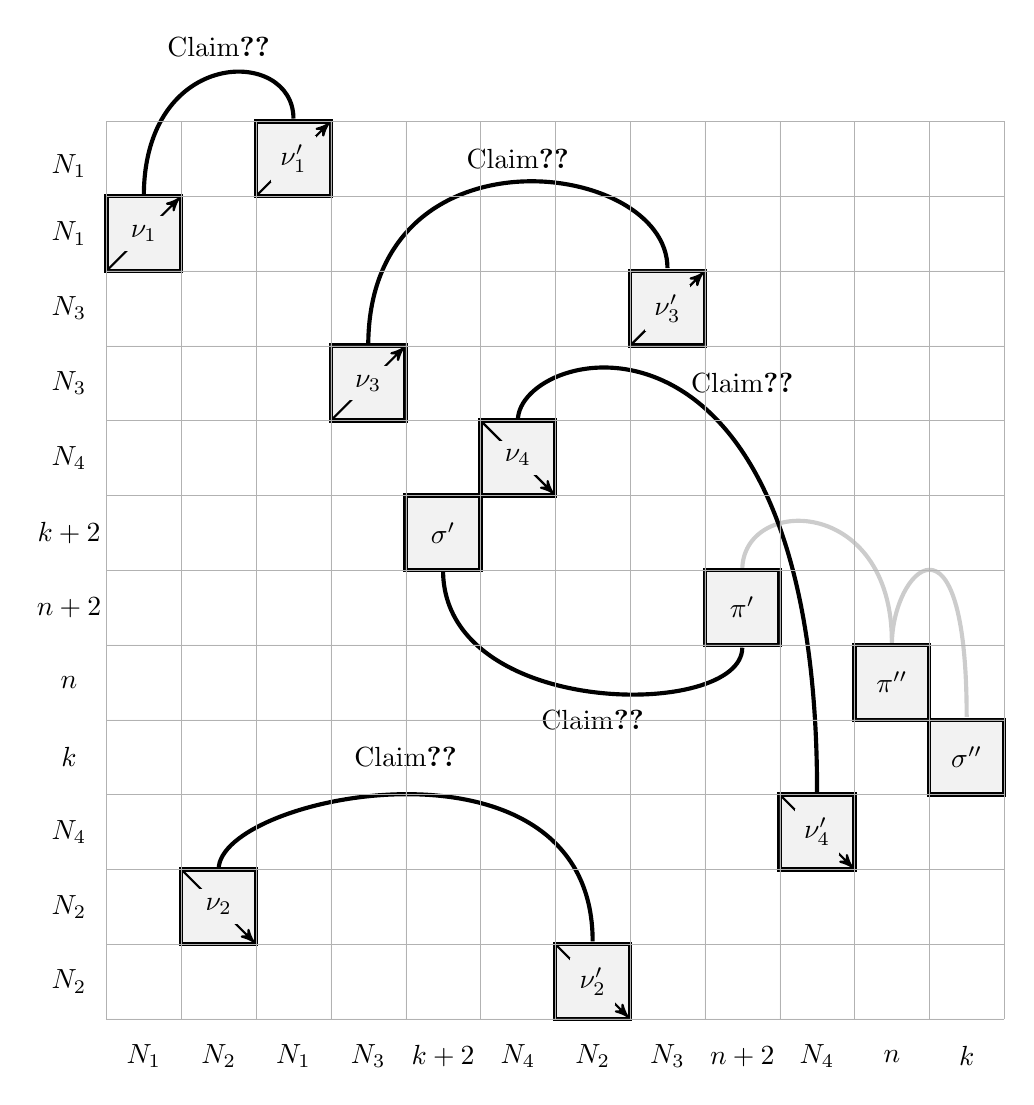
\begin{tikzpicture}[
      scale=.95,
      >=stealth',
      shorten >=1pt,
      main node/.style={align=center},
      cell/.style={draw,ultra thick,fill=black!5},
      structure link/.style={line width=1.5pt},
      pattern link/.style={line width=1.5pt,black!20},
      monotone/.style={->,thick}
      ]
      % edges
      % pi 1 - pi 2
      \draw [pattern link] (8.5,6) .. controls +(0,1) and +(0,2) .. (10.5,5);
      % pi 2 - sigma 2
      \draw [pattern link] (10.5,5) .. controls +(0,1) and +(0,3) .. (11.5,4);
      % 1
      \draw [structure link] (0.5,11) .. controls +(0,2) and +(0,1) .. (2.5,12);
      \node (claim edge 1) at (1.5,13) {Claim\ref{}};
      % 2
      \draw [structure link] (1.5,2) .. controls +(0,1) and +(0,3) .. (6.5,1);
      \node (claim edge 1) at (4,3.5) {Claim\ref{}};
      % 3
      \draw [structure link] (3.5,9) .. controls +(0,3) and +(0,1.5) .. (7.5,10);
      \node (claim edge 1) at (5.5,11.5) {Claim\ref{}};
      % 4
      \draw [structure link] (5.5,8) .. controls +(0,1) and +(0,7) .. (9.5,3);
      \node (claim edge 1) at (8.5,8.5) {Claim\ref{}};
      % sigma 1 - pi 1
      \draw [structure link] (4.5,6) .. controls +(0,-2) and +(0,-1) .. (8.5,5);
      \node (claim edge 1) at (6.5,4) {Claim\ref{}};
      % nodes
      % 1
      \draw [cell] (0,10) -- (1,10) -- (1,11) -- (0,11) -- cycle;
      \draw [monotone] (0,10) -- ++(1,1) node [midway,fill=white,fill=black!5] {$\nu_1$};
      %\draw [draw,ultra thick,fill=black!5] (0,10) -- (1,10) -- (1,11) -- (0,11) -- cycle;
      \draw [cell] (2,11) -- (3,11) -- (3,12) -- (2,12) -- cycle;
      \draw [monotone] (2,11) -- ++(1,1) node [midway,fill=white,fill=black!5] {$\nu'_1$};
      % 2
      \draw [cell] (1,1) -- (2,1) -- (2,2) -- (1,2) -- cycle;
      \draw [monotone] (1,2) -- ++(1,-1) node [midway,fill=white,fill=black!5] {$\nu_2$};
      \draw [cell] (6,0) -- (7,0) -- (7,1) -- (6,1) -- cycle;
      \draw [monotone] (6,1) -- ++(1,-1) node [midway,fill=white,fill=black!5] {$\nu'_2$};
      % 3
      \draw [cell] (3,8) -- (4,8) -- (4,9) -- (3,9) -- cycle;
      \draw [monotone] (3,8) -- ++(1,1) node [midway,fill=white,fill=black!5] {$\nu_3$};
      \draw [cell] (7,9) -- (8,9) -- (8,10) -- (7,10) -- cycle;
      \draw [monotone] (7,9) -- ++(1,1) node [midway,fill=white,fill=black!5] {$\nu'_3$};
      % 4
      \draw [cell] (5,7) -- (6,7) -- (6,8) -- (5,8) -- cycle;
      \draw [monotone] (5,8) -- ++(1,-1) node [midway,fill=white,fill=black!5] {$\nu_4$};
      \draw [cell] (9,2) -- (10,2) -- (10,3) -- (9,3) -- cycle;
      \draw [monotone] (9,3) -- ++(1,-1) node [midway,fill=white,fill=black!5] {$\nu'_4$};
      % sigma 1
      \draw [cell] (4,6) -- (5,6) -- (5,7) -- (4,7) -- cycle;
      \node [main node] (sigma1) at (4.5,6.5) {$\sigma'$};
      % pi 1
      \draw [cell] (8,5) -- (9,5) -- (9,6) -- (8,6) -- cycle;
      \node [main node] (pi1) at (8.5,5.5) {$\pi'$};
      % pi 2
      \draw [cell] (10,4) -- (11,4) -- (11,5) -- (10,5) -- cycle;
      \node [main node] (sigma2) at (10.5,4.5) {$\pi''$};
      % sigma 2
      \draw [cell] (11,3) -- (12,3) -- (12,4) -- (11,4) -- cycle;
      \node [main node] (pi2) at (11.5,3.5) {$\sigma''$};
      % grid
      \draw[step=1cm,black!30,ultra thin,fill=black!10] (0,0) grid (12,12);
      % row size
      \foreach \y/\N in {0.5/N_2,1.5/N_2,2.5/N_4,3.5/k,4.5/n,5.5/n+2,6.5/k+2,7.5/N_4,8.5/N_3,9.5/N_3,10.5/N_1,11.4/N_1} {
          \node at (-0.5,\y) (R\y) {$\N$};
      }
      % column size
      \foreach \x/\N in
      {0.5/N_1,1.5/N_2,2.5/N_1,3.5/N_3,4.5/k+2,5.5/N_4,6.5/N_2,7.5/N_3,8.5/n+2,9.5/N_4,10.5/n,11.5/k} {
          \node at (\x,-0.5) (C\x) {$\N$};
      }
    \end{tikzpicture}
    \caption{\label{fig:reduction}}
  \end{figure}


  \begin{align*}
  N_4 &= 2(2n + k + 2) + 1  = 4n + 2k + 5 \\
  N_3 &= 2(2N_4 + 2n + 2k + 4) + 1 = 20n + 12k + 9 \\
  N_2 &= 2(2N_3 + 2N_4 + 2n + 2k + 4) + 1 \\
  N_1 &= 2(2N_2 + 2N_3 + 2N_4 + 2n + 2k + 4) + 1\text{.}
  \end{align*}
  Notice that $N_1, N_2, N_3$ and $N_4$ are polynomial in $n$.
  The crucial properties are that
  (i) $N_1, N_2, N_3$ and $N_4$ are odd integers
  and
  (ii) $N_i > \left(\sum_{i < j \leq 4} 2N_j\right) + 2n + 2k + k$
  for every $1 \leq i \leq 4$.

  We now turn to defining various gadgets (sequences of integers)
  that act as building blocks in our construction:
  \begin{align*}
  \sigma'  &= ((k+1) \; \sigma \; (k+2)) \; [2N_2 + N_4 + 2n + k + 2] \\
  \pi'     &= ((n+1) \; \pi \; (n+2)) \; [2N_2 + N_4 + n + k + 2] \\
  \sigma'' &= \sigma \; [2N_2 + N_4] \\
  \pi''    &= \pi \; [2N_2 + N_4 + k] \\
  \nu_1    &= \nearrow_{N_1} \; [2N_2 + 2N_3 + 2N_4 + 2n + 2k + 4] \\
  \nu'_1   &= \nearrow_{N_1} \; [N_1 + 2N_2 + 2N_3 + 2N_4 + 2n + 2k + 4] \\
  \nu_2    &= \nearrow_{N_2} \; [N_2] \\
  \nu'_2   &= \searrow_{N_2} \\
  \nu_3    &= \nearrow_{N_3} \; [2N_2 + 2N_4 + 2n + 2k + 4] \\
  \nu'_3   &= \nearrow_{N_3} \; [2N_2 + N_3 + 2N_4 + 2n + 2k + 4] \\
  \nu_4    &= \searrow_{N_4} \; [2N_2 + N_4 + 2n + 2k + 4] \\
  \nu'_4   &= \searrow_{N_4} \; [2N_2]\text{.}
  \end{align*}
  We are now in position to define our target permutation $\mu$:
  $$
  \mu
  =
  \nu_1 \; \nu_2 \; \nu'_1 \; \nu_3 \; \sigma' \; \nu_4 \; \nu'_3 \; \pi' \; \nu'_4 \; \pi'' \; \sigma''
  \text{.}
  $$
  We claim that $\sigma$ occurs as a pattern in $\pi$ if and only if
  there exists a containment-free perfect matching
  $\mathcal{M}$ in $G_\mu$ such that
  for any two disctinct edges
  $(a, b)$ and $(a', b')$ in $\mathcal{M}$
  we have $\mu(a) < \mu(a')$ if and only if $\mu(b) < \mu(b')$.

  Suppose first that $\sigma$ occurs in $\pi$ as a pattern.
  We show how to construct a containment-free perfect matching
  $\mathcal{M}$ in $G_\mu$ such that
  for any two disctinct edges
  $(a, b)$ and $(a', b')$ in $\mathcal{M}$
  we have $\mu(a) < \mu(a')$ if and only if $\mu(b) < \mu(b')$.
  \begin{itemize}
    \item $\mathcal{M}$ contains $N_1$ pairwise crossing
    $(\nu_1, \nu'_1)$-edges.
    \item $\mathcal{M}$ contains $N_2$ pairwise crossing
    $(\nu_2, \nu'_2)$-edges.
    \item $\mathcal{M}$ contains $N_3$ pairwise crossing
    $(\nu_3, \nu'_3)$-edges.
    \item $\mathcal{M}$ contains $N_4$ pairwise crossing
    $(\nu_4, \nu'_4)$-edges.
    \item $\mathcal{M}$ contains $k+2$ pairwise crossing
    $(\sigma', \pi')$-edges as depicted in Figure~\ref{}.
    (Notice that we use here the fact that $\sigma$ occurs as a pattern in $\pi$).
    \item $\mathcal{M}$ contains $n-k$ pairwise crossing
    $(\pi', \pi'')$-edges as depicted in Figure~\ref{}.
    \item $\mathcal{M}$ contains $k$ pairwise crossing
    $(\pi'', \sigma'')$-edges as depicted in Figure~\ref{}.
    (Notice that we use here again the fact that $\sigma$ occurs as a pattern in $\pi$).
  \end{itemize}
  It can be easily checked (probably referring to Figure~\ref{}) that
  $\mathcal{M}$ is perfect and that
  for any two disctinct edges
  $(a, b)$ and $(a', b')$ in $\mathcal{M}$
  we have $\mu(a) < \mu(a')$ if and only if $\mu(b) < \mu(b')$.


    \begin{figure}[t!]
      \centering
        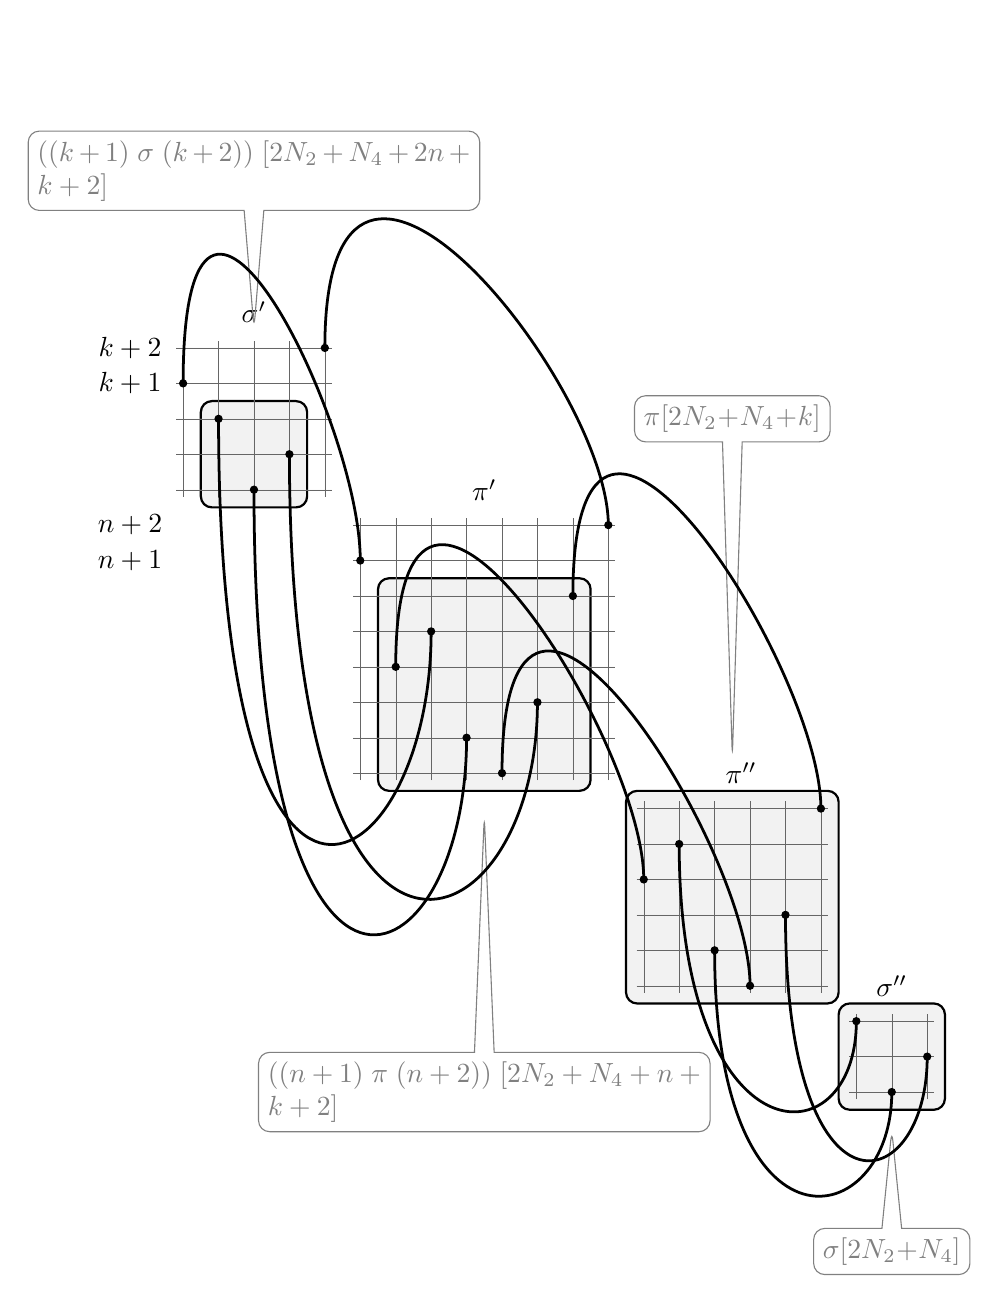
\begin{tikzpicture}
          [
            scale=0.45,
            label/.style={anchor=base},
            cell/.style={draw,thick,fill=black!5}
          ]
          % sigma'
          \draw [cell,rounded corners] (1.5,16.5) -- (4.5,16.5) -- (4.5,19.5) -- (1.5,19.5) -- cycle;
          \draw[step=1cm,black!60,ultra thin,fill=black!10] (0.8,16.8) grid (5.2,21.2);
          \foreach \x/\y in {1/20,2/19,3/17,4/18,5/21} {
              \draw [fill=black] (\x,\y) circle (0.1);
          }
          \node (pip) at (3,22) {$\sigma'$};
          \node[%
            draw,
            text width=5.5cm,text justified,color=black!50,rounded corners,
            rectangle callout,callout relative pointer={(0.0cm,-1.5cm)}
          ] at (3,26)
          {%
            $((k+1) \; \sigma \; (k+2)) \; [2N_2 + N_4 + 2n + k + 2]$
          };%
          %\node at (3,-0.5) {$((k+1) \; \sigma \; (k+2)) \; [2N_2 + N_4 + 2n + k + 2]$};
          \node at (-0.5,20) {$k+1$};
          \node at (-0.5,21) {$k+2$};
          % pi'
          \draw [cell,rounded corners] (6.5,8.5) -- (12.5,8.5) -- (12.5,14.5) -- (6.5,14.5) -- cycle;
          \draw[step=1cm,black!60,ultra thin,fill=black!10] (5.8,8.8) grid (13.2,16.2);
          \foreach \x/\y in {6/15,7/12,8/13,9/10,10/9,11/11,12/14,13/16} {
              \draw [fill=black] (\x,\y) circle (0.1);
          }
          \node (pip) at (9.5,17) {$\pi'$};
          \node[%
            draw,
            text width=5.5cm,text justified,color=black!50,rounded corners,
            rectangle callout,callout relative pointer={(0.0cm,3cm)}
          ] at (9.5,0)
          {%
            $((n+1) \; \pi \; (n+2)) \; [2N_2 + N_4 + n + k + 2]$
          };%
          %\node at (9.5,-2) {$((n+1) \; \pi \; (n+2)) \; [2N_2 + N_4 + n + k + 2]$};
          \node at (-0.5,15) {$n+1$};
          \node at (-0.5,16) {$n+2$};
          % pi''
          \draw [cell,rounded corners] (13.5,2.5) -- (19.5,2.5) -- (19.5,8.5) -- (13.5,8.5) -- cycle;
          \draw[step=1cm,black!60,ultra thin,fill=black!10] (13.8,2.8) grid (19.2,8.2);
          \foreach \x/\y in {14/6,15/7,16/4,17/3,18/5,19/8} {
              \draw [fill=black] (\x,\y) circle (0.1);
          }
          \node (pipp) at (16.75,9) {$\pi''$};
          \node[%
            draw,
            text width=2.25cm,text justified,color=black!50,rounded corners,
            rectangle callout,callout relative pointer={(0.0cm,-4cm)}
          ] at (16.5,19)
          {%
            $\pi [2N_2 + N_4 + k]$
          };%
          %\node at (16.5,-3.5) {$\pi [2N_2 + N_4 + k]$};
          % sigma''
          \draw [cell,rounded corners] (19.5,-0.5) -- (22.5,-.5) -- (22.5,2.5) -- (19.5,2.5) -- cycle;
          \draw[step=1cm,black!60,ultra thin,fill=black!10] (19.8,-0.2) grid (22.2,2.2);
          \foreach \x/\y in {20/2,21/0,22/1} {
              \draw [fill=black] (\x,\y) circle (0.1);
          }
          \node (sigmapp) at (21,3) {$\sigma''$};
          \node[%
            draw,
            text width=1.75cm,text justified,color=black!50,rounded corners,
            rectangle callout,callout relative pointer={(0.0cm,1.25cm)}
          ] at (21,-4.5)
          {%
            $\sigma [2N_2 + N_4]$
          };%
          %\node at (21,-5) {$\sigma [2N_2 + N_4]$};
          % edges sigma' - pi'
          \draw [line width=1pt]
          (1,20) .. controls +(0,9) and +(0,4) .. (6,15);
          \draw [line width=1pt]
          (5,21) .. controls +(0,9) and +(0,4) .. (13,16);
          \draw [line width=1pt]
          (2,19) .. controls +(0,-17) and +(0,-7) .. (8,13);
          \draw [line width=1pt]
          (3,17) .. controls +(0,-17) and +(0,-7) .. (9,10);
          \draw [line width=1pt]
          (4,18) .. controls +(0,-17) and +(0,-7) .. (11,11);
          % edges pi' - pi''
          \draw [line width=1pt]
          (7,12) .. controls +(0,9) and +(0,4) .. (14,6);
          \draw [line width=1pt]
          (10,9) .. controls +(0,9) and +(0,4) .. (17,3);
          \draw [line width=1pt]
          (12,14) .. controls +(0,9) and +(0,4) .. (19,8);
          % edges pi'' - sigma''
          \draw [line width=1pt]
          (15,7) .. controls +(0,-9) and +(0,-4) .. (20,2);
          \draw [line width=1pt]
          (16,4) .. controls +(0,-9) and +(0,-4) .. (21,0);
          \draw [line width=1pt]
          (18,5) .. controls +(0,-9) and +(0,-4) .. (22,1);
          % text
          % \node[%
          %   draw,
          %   text width=5.5cm,text justified,color=black!50,
          %   rectangle callout,callout relative pointer={(0.5cm,-.75cm)}
          % ] at (1,27)
          % {%
          % $2$ pairwise crossing $(\sigma',\pi')$-edges that
          % link the guards
          % };%
          % \node[%
          %   draw,
          %   text width=5.5cm,text justified,color=black!50,
          %   rectangle callout,callout relative pointer={(-0.1cm,-2.5cm)}
          % ] at (17,24)
          % {%
          % $n-k$ pairwise crossing $(\sigma',\pi')$-edges that
          % denote positions that do not correspond to
          % a specific occurence of $\sigma$ in $\pi$
          % (at positions $2$, $3$ and $5$).
          % };%
          % \node[%
          %   draw,
          %   text width=5.5cm,text justified,color=black!50,
          %   rectangle callout,callout relative pointer={(0.75cm,1.5cm)}
          % ] at (2.5,4,5)
          % {%
          % $k$ pairwise crossing $(\sigma',\pi')$-edges that
          % denote a specific occurence of $\sigma$ in $\pi$
          % (at positions $2$, $3$ and $5$).
          % };%
          % \node[%
          %   draw,
          %   text width=5.5cm,text justified,color=black!50,
          %   rectangle callout,callout relative pointer={(2cm,.75cm)}
          % ] at (7,-3)
          % {%
          % $k$ pairwise crossing $(\pi''; \sigma'')$-edges that
          % denote a specific occurence of $\sigma$ in $\pi$
          % (at positions $2$, $3$ and $5$).
          % };%
        \end{tikzpicture}
        \caption{\label{fig:subfig:sigma' - pi' - pi'' - sigma''}%
        $\sigma = 312$ and $\pi = 4\mathbf{5}\mathbf{2}1\mathbf{3}6$
        (where a specific occurrence of $\sigma$ in $\pi$ is depicted in bold).
        }
      \end{figure}

  More precisely,
  (i) the first integer of $\sigma'$
  (\emph{i.e.}, $(k+1) + (2N_2 + N_4 + 2n + k + 2)$) is linked
  to the first integer of $\pi'$
  ((\emph{i.e.}, $(n+1) + (2N_2 + N_4 + n + k + 2)$)),
  (ii)

  (this is possible since ).
  Conversely, suppose that there exists a containment-free perfect matching
  $\mathcal{M}$ in $G_\mu$ such that for any two disctinct edges
  $(a, b)$ and $(a', b')$ in $\mathcal{M}$
  we have $\mu(a) < \mu(a')$ if and only if $\mu(b) < \mu(b')$.
  We show that $\sigma$ occurs as a pattern in $\pi$.
  Whereas the matching $\mathcal{M}$ may not be as regular as in the forward
  direction, the main idea is to prove that $\mathcal{M}$ contains enough structure
  (more precisely, enough $(\sigma', \pi')$-edges) so that we can conclude.
  We have divided the reverse direction into a serie of basic claims that
  progressively defines the overall structure of $\mathcal{M}$.


    \begin{figure}[t!]
      \centering
      \subfigure[%
        A $(\nu_1, \nu_2)$-edge $(a, b)$ together with a
        $(\nu_2, \nu'_1)$-edge $(x, y)$.
        Notice that we may have $x<b$
        (as long as $N_1 < x \leq N_1+N_2$ and $N_1 < b \leq N_1+N_2$
        do hold).
      ]{%
        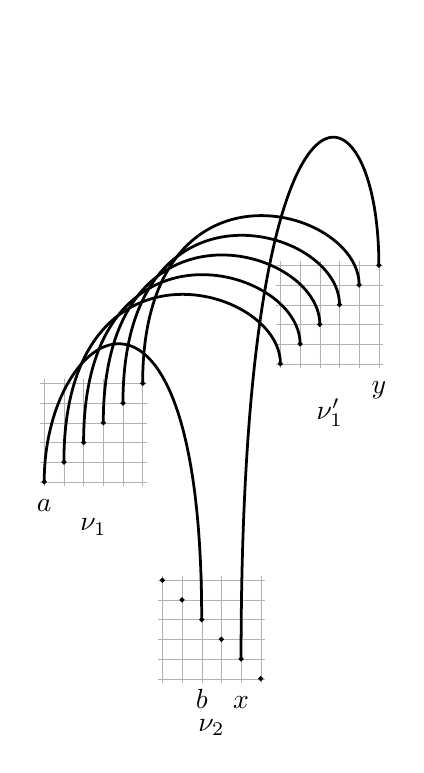
\begin{tikzpicture}
          [
            scale=0.25,
            label/.style={anchor=base}
          ]
          % nu_1
          \draw[step=1cm,black!30,ultra thin,fill=black!10] (-0.2,9.8) grid (5.2,15.2);
          \foreach \x/\y in {0/10,1/11,2/12,3/13,4/14,5/15} {
              \draw [fill=black] (\x,\y) circle (0.1);
          }
          % nu_4
          \draw[step=1cm,black!30,ultra thin,fill=black!10] (5.8,-0.2) grid (11.2,5.2);
          \foreach \x/\y in {6/5,7/4,8/3,9/2,10/1,11/0} {
              \draw [fill=black] (\x,\y) circle (0.1);
          }
          % nu'_1
          \draw[step=1cm,black!30,ultra thin,fill=black!10] (11.8,15.8) grid (17.2,21.2);
          \foreach \x/\y in {12/16,13/17,14/18,15/19,16/20,17/21} {
              \draw [fill=black] (\x,\y) circle (0.1);
          }
          % labels
          \node [label] (x) at (17,14.5) {$y$};
          \node [label] (x) at (10,-1.5) {$x$};
          \node [label] (a) at (0,8.5) {$a$};
          \node [label] (b) at (8,-1.5) {$b$};
          \node (nu1) at (2.5,7.7) {$\nu_1$};
          \node (nu2) at (8.5,-2.5) {$\nu_2$};
          \node (nu1') at (14.5,13.5) {$\nu'_1$};
          % crossings edges
          \draw [line width=1pt]
          (1,11) .. controls +(0,12) and +(0,4) .. (12,16);
          \draw [line width=1pt]
          (2,12) .. controls +(0,12) and +(0,4) .. (13,17);
          \draw [line width=1pt]
          (3,13) .. controls +(0,12) and +(0,4) .. (14,18);
          \draw [line width=1pt]
          (4,14) .. controls +(0,12) and +(0,4) .. (15,19);
          \draw [line width=1pt]
          (5,15) .. controls +(0,12) and +(0,4) .. (16,20);
          % data edges
          \draw [line width=1pt]
          (0,10) .. controls +(0,8) and +(0,20) .. (8,3);
          \draw [line width=1pt]
          (10,1) .. controls +(0,32) and +(0,10) .. (17,21);
        \end{tikzpicture}
        \label{subfig:no (nu_1, nu_2)-edge - 1}
      }% end subfigure
      \qquad
      \subfigure[%
        A $(\nu_1, \nu'_1)$-edge $(x', y')$ together with an
        edge $(y, z)$ which is neither
        a $(\nu_1, \nu'_1)$-edge,
        nor a $(\nu_2, \nu'_1)$-edge,
        nor a $(\nu'_1, \nu'_1)$-edge.
        Notice that $y$ may be any position satisfying
        $N_1+N_2 < y \leq 2N_1+N_2$.
      ]{%
      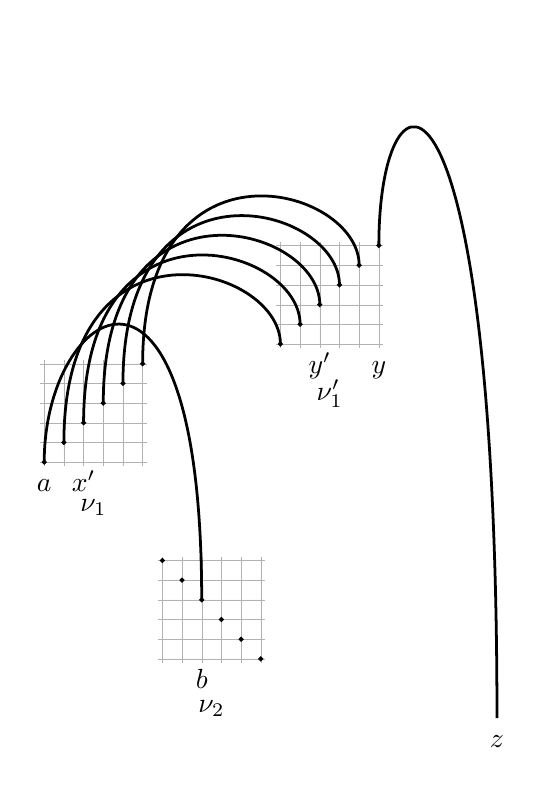
\begin{tikzpicture}
        [
          scale=0.25,
          label/.style={anchor=base}
        ]
        % nu_1
        \draw[step=1cm,black!30,ultra thin,fill=black!10] (-0.2,9.8) grid (5.2,15.2);
        \foreach \x/\y in {0/10,1/11,2/12,3/13,4/14,5/15} {
            \draw [fill=black] (\x,\y) circle (0.1);
        }
        % nu_4
        \draw[step=1cm,black!30,ultra thin,fill=black!10] (5.8,-0.2) grid (11.2,5.2);
        \foreach \x/\y in {6/5,7/4,8/3,9/2,10/1,11/0} {
            \draw [fill=black] (\x,\y) circle (0.1);
        }
        % nu'_1
        \draw[step=1cm,black!30,ultra thin,fill=black!10] (11.8,15.8) grid (17.2,21.2);
        \foreach \x/\y in {12/16,13/17,14/18,15/19,16/20,17/21} {
            \draw [fill=black] (\x,\y) circle (0.1);
        }
        % labels
        \node [label] (x) at (17,14.5) {$y$};
        \node [label] (x) at (23,-4.5) {$z$};
        \node [label] (a) at (0,8.5) {$a$};
        \node [label] (a) at (2,8.5) {$x'$};
        \node [label] (a) at (14,14.5) {$y'$};
        \node [label] (b) at (8,-1.5) {$b$};
        \node (nu1) at (2.5,7.7) {$\nu_1$};
        \node (nu2) at (8.5,-2.5) {$\nu_2$};
        \node (nu1') at (14.5,13.5) {$\nu'_1$};
        % crossings edges
        \draw [line width=1pt]
        (1,11) .. controls +(0,12) and +(0,4) .. (12,16);
        \draw [line width=1pt]
        (2,12) .. controls +(0,12) and +(0,4) .. (13,17);
        \draw [line width=1pt]
        (3,13) .. controls +(0,12) and +(0,4) .. (14,18);
        \draw [line width=1pt]
        (4,14) .. controls +(0,12) and +(0,4) .. (15,19);
        \draw [line width=1pt]
        (5,15) .. controls +(0,12) and +(0,4) .. (16,20);
        % data edges
        \draw [line width=1pt]
        (0,10) .. controls +(0,8) and +(0,20) .. (8,3);
        \draw [line width=1pt]
        (17,21) .. controls +(0,10) and +(0,35) .. (23,-3);
        \end{tikzpicture}
        \label{subfig:no (nu_1, nu_2)-edge - 2}
      }% end subfigure
      \caption{\label{fig:subfig:no (nu_1, nu_2)-edge}%
        Claim~\ref{claim:no (nu_1, nu_2)-edge}:
        Assuming a $(\nu_1,\nu_2)$-edge $(a, b)$ in $\mathcal{M}$.
      }
    \end{figure}

  \begin{claim}
    \label{claim:no (nu_1, nu_2)-edge}
    There is no $(\nu_1, \nu_2)$-edge in $\mathcal{M}$.
  \end{claim}

  \begin{proof}[of Claim~\ref{claim:no (nu_1, nu_2)-edge}]
    We first prove that there exists at most one
    $(\nu_1, \nu_2)$-edge in $\mathcal{M}$.
    Indeed, suppose, aiming at a contradiction, that there exist
    two $(\nu_1, \nu_2)$-edges $e = (a, b)$ and $e' = (a', b')$ in $\mathcal{M}$.
    Since $\mathcal{M}$ is containment-free,
    we may assume that $a < a'$ and $b < b'$.
    Then it follows that $\mu(a) < \mu(a')$
    (since $\nu_1$ is increasing) and $\mu(b) > \mu(b')$
    (since $\nu_2$ is decreasing),
    which contradicts our hypothesis.

    Suppose now, still aiming at a contradiction, that there exists
    exactly one $(\nu_1, \nu_2)$-edge $e = (a, b)$ in $\mathcal{M}$.
    We show that $\mathcal{M}$ does not contain any $(\nu_1, \nu_1)$-edge.
    Indeed, suppose, aiming at a contradiction,
    that there exists a $(\nu_1, \nu_1)$-edge $(x, y)$ in $\mathcal{M}$.
    Since $\mathcal{M}$ is containment-free,
    we must have $x < a$.
    Then it follows that $\mu(x) < \mu(a)$ (since $\nu_1$ is increasing) and
    $\mu(y) > \mu(b)$ (since $\nu_1$ is above $\nu_2$),
    which contradicts our hypothesis.
    Hence $\mathcal{M}$ does not contain any $(\nu_1, \nu_1)$-edge.
    Furthermore, since $\nu_1$ is increasing and
    there exists only one $(\nu_1, \nu_2)$-edge in $\mathcal{M}$,
    we conclude that
    $\mathcal{M}$ contains $N_1-1$ pairwise crossing $(\nu_1, \nu'_1)$-edges.
    But $|\nu_1| = |\nu'_1| = N_1$ and $\mathcal{M}$ is perfect,
    and hence there exists a position, say $y$, in $\nu'_1$ that is
    not involved in a $(\nu_1, \nu'_1)$-edge in $\mathcal{M}$.
    We rule out this configuration by considering two cases:
    \begin{itemize}
      \item Position $y$ is involved in a $(\nu_2, \nu'_1)$-edge,
      say $(x, y)$. Then, we have $\mu(a) > \mu(x)$ (since $\nu_1$ is above $\nu_2$)
      and $\mu(b) < \mu(y)$ (since $\nu_2$ is below $\nu'_1$),
      which contradicts our hypothesis.
      See Fig.~\ref{subfig:no (nu_1, nu_2)-edge - 1}.
      \item Position $y$ is not involved in a $(\nu_2, \nu'_1)$-edge.
      Since $\mathcal{M}$ contains $N_1-1$ pairwise crossing $(\nu_1, \nu'_1)$-edges
      in $\mathcal{M}$ and $|\nu'_1| = N_1$, there exists an edge $(y, z)$ in $\mathcal{M}$
      that is neither a $(\nu_1, \nu'_1)$-edge nor a $(\nu_2, \nu'_1)$-edge
      nor a $(\nu'_1, \nu'_1)$-edge.
      In other words, $z > 2N_1 + N_2$.
      Now, for any $(\nu_1, \nu'_1)$-edge $(x', y')$ in $\mathcal{M}$, we
      have $\mu(x') < \mu(y)$ (since $\nu_1$ is below $\nu'_1$)
      and $\mu(y') > \mu(z)$ (since $\nu'_1$ is above any other gadget),
      which contradicts our hypothesis.
      See Fig.~\ref{subfig:no (nu_1, nu_2)-edge - 2}.
    \end{itemize}
    \qed
  \end{proof}



  \begin{claim}
    \label{claim:one (nu_1, nu'_1)-edge}
    There is at least one $(\nu_1, \nu'_1)$-edge in $\mathcal{M}$.
  \end{claim}

  \begin{proof}[of Claim~\ref{claim:one (nu_1, nu'_1)-edge}]
    Suppose, aiming at a contradiction, that there is no
    $(\nu_1, \nu'_1)$-edge in $\mathcal{M}$.
    Then it follows that there exists an edge $(x, y)$ in $\mathcal{M}$,
    $1 \leq x \leq N_1$, that is neither a
    $(\nu_1, \nu_1)$-edge (since $N_1$ is odd)
    nor a $(\nu_1, \nu_2)$-edge (Claim~\ref{claim:no (nu_1, nu_2)-edge})
    nor a $(\nu_1, \nu'_1)$ (by our contradiction hypothesis).
    (In other words, $x \leq N_1$ and $y > 2N_1 + N_2$.)
    Therefore, since $\mathcal{M}$ is containment-free,
    there is neither a $(\nu_2, \nu_2)$-edge nor a $(\nu'_1, \nu'_1)$-edge
    in $\mathcal{M}$.
    Then it follows that every position $x$ of $\nu'_1$
    (\emph{i.e.}, $N_1+N_2 < x \leq 2N_1+N_2$)
    is involved in an edge $(x, y)$ of $\mathcal{M}$ with $y \geq 2N_1+N_2$.
    But $|\nu'_1| = N_1 = 2(2N_2 + 2n_3 + 2N_4 + 2n + 2k + 4) + 1
    > 2N_2 + 2N_3 + 2N_4 + 2n + 2k + 4$, and hence at least one
    position in $\nu'_1$ can not be involved in an edge in $\mathcal{M}$.
    Then it follows that $\mathcal{M}$ is not a perfect matching,
    which contradicts our hypothesis.
    \qed
  \end{proof}

  \begin{claim}
    \label{claim:no (nu_2, nu_2)-edge}
    There is no $(\nu_2, \nu_2)$-edge in $\mathcal{M}$.
  \end{claim}

  \begin{proof}[of Claim~\ref{claim:no (nu_2, nu_2)-edge}]
  Combine the fact that $\mathcal{M}$ is containment-free with
  Claim~\ref{claim:one (nu_1, nu'_1)-edge}.
  \qed
  \end{proof}

  \begin{claim}
    \label{claim:no (nu_2, nu'_1)-edge}
    There is no $(\nu_2, \nu'_1)$-edge in $\mathcal{M}$.
  \end{claim}

  \begin{proof}[of Claim~\ref{claim:no (nu_2, nu'_1)-edge}]
    We first prove that there exists at most one
    $(\nu_2, \nu'_1)$-edge in $\mathcal{M}$.
    Indeed, suppose, aiming at a contradiction, that there exist
    two $(\nu_2, \nu'_1)$-edges $e = (a, b)$ and $e' = (a', b')$ in $\mathcal{M}$.
    Since $\mathcal{M}$ is containment-free,
    we may assume that $a < a'$ and $b < b'$.
    Then it follows that $\mu(a) > \mu(a')$
    (since $\nu_2$ is decreasing) and $\mu(b) < \mu(b')$
    (since $\nu'_1$ is increasing),
    which contradicts our hypothesis.

    Suppose now, still aiming at a contradiction, that there exists
    exactly one $(\nu_2, \nu'_1)$-edge $e = (a, b)$ in $\mathcal{M}$.
    According to Claim~\ref{claim:one (nu_1, nu'_1)-edge}, there exists at least
    one $(\nu_1, \nu'_1)$-edge in $\mathcal{M}$.
    Furtheremore, since
    there is no $(\nu_1, \nu_2)$-edge (Claim~\ref{claim:no (nu_1, nu_2)-edge}),
    every position in $\nu_1$ is involved either in a
    $(\nu_1, \nu_1)$-edge or in a $(\nu_1, \nu'_1)$-edge in $\mathcal{M}$
    (otherwise $\mathcal{M}$ would not be containment-free).
    Then it follows that that there is an odd number of $(\nu_1, \nu'_1)$-edges
    in $\mathcal{M}$ since $\mathcal{M}$ is perfect and $|\nu_1| = N_1$ is odd.
    Combining this with the fact that there exists exactly one $(\nu_2, \nu'_1)$-edge
    in $\mathcal{M}$ and $|\nu'_1| = N_1$ is odd,
    we conclude that there exists a position, say $x$, in $\nu'_1$
    that is neither involved in a $(\nu_1, \nu'_1)$-edge nor a $(\nu_1, \nu'_1)$-edge
    nor a $(\nu'_1, \nu'_1)$-edge.
    Write $(x, y)$, $N_1+N_2 < x \leq 2N_1 + N_2$ and $y > 2N_1 + N_2$, this edge.
    We have $\mu(a) < \mu(x)$ (since $\nu_2$ is below $\nu'_1$)
    and $\mu(b) > \mu(y)$ (since $\nu'_1$ is above any other gadget),
    which contradicts our hypothesis.
    \qed
  \end{proof}

  \begin{claim}
    \label{claim:one (nu_2, nu'_2)-edge}
    There is at least one $(\nu_2, \nu'_2)$-edge in $\mathcal{M}$.
  \end{claim}

  \begin{proof}[of Claim~\ref{claim:one (nu_2, nu'_2)-edge}]
    Suppose, aiming at a contradiction there there is no
    $(\nu_2, \nu'_2)$-edge in $\mathcal{M}$.
    Notice that there is no
    $(\nu_1, \nu_2)$-edge (Claim~\ref{claim:no (nu_1, nu_2)-edge})
    nor $(\nu_2, \nu_2)$-edge (Claim~\ref{claim:no (nu_2, nu_2)-edge})
    nor $(\nu_2, \nu'_1)$-edge (Claim~\ref{claim:no (nu_2, nu'_1)-edge})
    in $\mathcal{M}$.
    But $|\nu_2| = N_2 > 2N_3 + 2N_4 + 2n + 2k$ and hence $\mathcal{M}$ is not
    a perfect matching.
    According to Proposition~\ref{proposition:matching}, this is
    a contradiction.
    \qed
  \end{proof}

  \begin{claim}
    \label{claim:no (nu'_1, nu'_1),(nu_3, nu_3),(sigma' ,sigma'),(nu_4, nu_4)-edge}
    There is
    no $(\nu'_1, \nu'_1)$-edge,
    no $(\nu_3, \nu_3)$-edge,
    no $(\sigma', \sigma')$-edge and
    no $(\nu_4, \nu_4)$-edge
    in $\mathcal{M}$.
  \end{claim}

  \begin{proof}[of Claim~\ref{claim:no (nu'_1, nu'_1),(nu_3, nu_3),(sigma' ,sigma'),(nu_4, nu_4)-edge}]
    Combine Claim~\ref{claim:one (nu_2, nu'_2)-edge} with the fact that
    $\mathcal{M}$ is containment-free (Proposition~\ref{proposition:matching}).
    \qed
  \end{proof}

  \begin{claim}
    \label{claim:no (nu_3, nu'_2)-edge}
    There is no $(\nu_3, \nu'_2)$-edge in $\mathcal{M}$.
  \end{claim}

  \begin{proof}[of Claim~\ref{claim:no (nu_3, nu'_2)-edge}]
    Suppose, aiming at a contradiction, that there exists
    $(\nu_3, \nu'_2)$-edge $(a, b)$ in $\mathcal{M}$.
    According to Claim~\ref{claim:one (nu_2, nu'_2)-edge}, there
    exists at least one $(\nu_2, \nu'_2)$-edge $(x, y)$ in $\mathcal{M}$.
    Since $\mathcal{M}$ is containment-free (Proposition~\ref{proposition:matching}),
    we have $y < b$.
    Therefore,
    we have $\mu(x) < \mu(a)$ (by construction) and
    $\mu(y) > \mu(b)$ (since $\nu'_2$ is decreasing).
    According to Proposition~\ref{proposition:matching}, this is
    a contradiction.
    \qed
  \end{proof}

  \begin{claim}
    \label{claim:no (nu_1, nu_3)-edge no (nu'_1, nu_3)-edge}
    There is neither $(\nu_1, \nu'_3)$-edge nor $(\nu'_1, \nu_3)$-edge
    in $\mathcal{M}$.
  \end{claim}

  \begin{proof}[of Claim~\ref{claim:no (nu_1, nu_3)-edge no (nu'_1, nu_3)-edge}]
    Suppose, aiming at a contradiction, that there exists a
    $(\nu_1, \nu'_3)$-edge $(a, b)$ in $\mathcal{M}$.
    According to Claim~\ref{claim:one (nu_1, nu'_1)-edge} there exists
    $(\nu_1, \nu'_1)$-edge $(x, y)$ in $\mathcal{M}$.
    Since these two edges have to be crossing
    (Proposition~\ref{proposition:matching}), we have $x < a$.
    Therefore, we have
    $\mu(x) < \mu(a)$ (since $\nu_1$ is increasing)
    and
    $\mu(y) > \mu(b)$ (by construction).
    According to Proposition~\ref{proposition:matching}, this is
    a contradiction.

    A similar argument shows that there is no
    $(\nu'_1, \nu_3)$-edge in $\mathcal{M}$.
    \qed
  \end{proof}

  \begin{claim}
    \label{claim:at most one (nu_2, nu_3)-edge}
    There is at most one $(\nu_2, \nu_3)$-edge
    in $\mathcal{M}$.
  \end{claim}

  \begin{proof}[of Claim~\ref{claim:at most one (nu_2, nu_3)-edge}]
    Suppose, aiming at a contradiction, that there exist two
    $(\nu_2, \nu_3)$-edges $(a, b)$ and $(a', b')$ in $\mathcal{M}$.
    Since these two edges have to be crossing
    (Proposition~\ref{proposition:matching}), we may assume that
    $a < a'$ and $b < b'$.
    Therefore, we have
    $\mu(a) > \mu(a')$ (since $\nu_2$ is decreasing)
    and
    $\mu(b) < \mu(b')$ (since $\nu_3$ is increasing).
    According to Proposition~\ref{proposition:matching}, this is
    a contradiction.
    \qed
  \end{proof}

  \begin{claim}
    \label{claim:one (nu_3, nu'_3)-edge}
    There is at least one $(\nu_3, \nu'_3)$-edge in $\mathcal{M}$.
  \end{claim}

  \begin{proof}[of Claim~\ref{claim:one (nu_3, nu'_3)-edge}]
    Suppose, aiming at a contradiction, that there is no
    $(\nu_3, \nu'_3)$-edge in $\mathcal{M}$.
    \qed
  \end{proof}

  \begin{claim}
    \label{claim:one (nu_4, nu'_4)-edge}
    There is at least one $(\nu_4, \nu'_4)$-edge in $\mathcal{M}$.
  \end{claim}

  \begin{proof}[of Claim~\ref{claim:one (nu_4, nu'_4)-edge}]
    Suppose, aiming at a contradiction, that there is no
    $(\nu_4, \nu'_4)$-edge in $\mathcal{M}$.
    \qed
  \end{proof}

  \begin{claim}
    \label{claim:no (nu_4, nu'_3)-edge}
    There is no $(\nu_4, \nu'_3)$-edge in $\mathcal{M}$.
  \end{claim}

  \begin{proof}[of Claim~\ref{claim:no (nu_4, nu'_3)-edge}]
    \qed
  \end{proof}

  \begin{claim}
    \label{claim:no (nu_4, pi')-edge}
    There is no $(\nu_4, \pi')$-edge in $\mathcal{M}$.
  \end{claim}

  \begin{proof}[of Claim~\ref{claim:no (nu_4, pi')-edge}]
    \qed
  \end{proof}

  \begin{claim}
    \label{claim:one (nu_4, nu'_4)-edge}
    There is at least $(\nu_4, \nu'_4)$-edge in $\mathcal{M}$.
  \end{claim}

  \begin{proof}[of Claim~\ref{claim:one (nu_4, nu'_4)-edge}]
    \qed
  \end{proof}

  \begin{claim}
    \label{claim:no (pi', pi'')-edge}
    There is no $(\pi', \pi'')$-edge in $\mathcal{M}$.
  \end{claim}

  \begin{proof}[of Claim~\ref{claim:no (pi', pi'')-edge}]
    \qed
  \end{proof}

  \begin{claim}
    \label{claim:no (nu'_2, pi')-edge}
    There is no $(\nu'_2, \pi')$-edge in $\mathcal{M}$.
  \end{claim}

  \begin{proof}[of Claim~\ref{claim:no (nu'_2, pi')-edge}]
    \qed
  \end{proof}

  \begin{claim}
    \label{claim:no (nu'_3, pi')-edge}
    There is no $(\nu'_3, \pi')$-edge in $\mathcal{M}$.
  \end{claim}

  \begin{proof}[of Claim~\ref{claim:no (nu'_3, pi')-edge}]
    \qed
  \end{proof}

  \begin{claim}
    \label{claim:no (nu_2, nu'_2)-edge}
    There is no $(\nu_2, \nu'_2)$-edge in $\mathcal{M}$.
  \end{claim}

  \begin{proof}[of Claim~\ref{claim:no (nu_2, nu'_2)-edge}]
    \qed
  \end{proof}

  \begin{claim}
    \label{claim:no (nu_3, nu'_3)-edge}
    There is no $(\nu_3, \nu'_3)$-edge in $\mathcal{M}$.
  \end{claim}

  \begin{proof}[of Claim~\ref{claim:no (nu_3, nu'_3)-edge}]
    \qed
  \end{proof}
\qed
\end{proof}

%%%%%%%%%%%%%%%%%%%%%%%%%%%%%%%%%%%%%%%%%%%%%%%%%%%%%%%%%%%%%%%%%%%%

%%
%% ---- Patterns ----
%%
\section{Patterns}
\label{section:Patterns}

\begin{proposition}
  \label{proposition:patterns:lower bound}
  Let $\pi \in S_{n}$.
  Then $\pi$ contains a pattern of size at least
  $\left\lfloor\sqrt{n-1}/2\right\rfloor$ that
  is the union of two order-isomorphic patterns.
\end{proposition}

\begin{proof}[of Proposition~\ref{proposition:patterns:lower bound}]
  The Erdös-Szekeres theorem \cite{Erdos:Szekeres:1935}
  states that every permutation of
  length at least $pq+1$ must contain either the pattern
  $\nearrow_{p+1}$ or the pattern $\searrow_{q+1}$.
  The result now follows from the fact that
  the pattern $\nearrow_{p+1}$ (resp. $\searrow_{q+1}$)
\qed
\end{proof}

\begin{proposition}
  \label{proposition:patterns:upper bound}
  If $2^{\binom{k}{2}} > \binom{n}{2k}\;\binom{2k}{k}$, then there exists
  a permutation of $S_{n}$
  that does not contains a pattern
  of length $2k$ that is the union of two
  order-isomorphic patterns.
\end{proposition}

\begin{proof}[of Proposition~\ref{proposition:patterns:upper bound}]
The proof is by the probabilistic method \cite{Alon:Spencer:1992}.
Let $\pi \in S_n$ be chosen randomly and uniformly.
For any pattern $\sigma$ of length $2k$ ($k$ to be precisely defined latter)
of $\pi$,
let $X_\sigma$ be the indicator variable that
$\sigma$ is the union of two order-ismorphic patterns.
According to Boole's inequality, we have
$P\left(X_\sigma\right) \leq \binom{2k}{k}\;2^{-k}$.
Since there are $\binom{n}{2k}$ patterns of length $2k$ in $\pi$,
the probability that $\pi$ contains a pattern of length $2k$
is the union of two order-ismorphic patterns is at most
$\binom{n}{2k}\;\binom{2k}{k}\;2^{-k} < 1$.
Thus, with positive probability, no event $X_\sigma$ occurs and
there is a permutation of $S_n$ that does not contain a pattern
of length $2k$ that is the union of two order-isomorphic patterns.
\qed
\end{proof}

\bigskip
\bigskip


Let $u$ be a binary word of length $n$ with $k$ occurrences of $0$.
We denote by $\BINTOPERM$ be the map sending any such word $u$ to the
permutation obtained by replacing from left to right each occurrence of
$0$ in $u$ by $1$, $2$, \dots, $k$, and from right to left each
occurrence of $1$ in $u$ by $k + 1$, $k + 2$, \dots, $n$. For instance,
\begin{equation}
    \BINTOPERM({\bf 1}00{\bf 1}0{\bf 1}{\bf 1}0{\bf 1}000) =
    {\bf C} 12 {\bf B} 3 {\bf A} {\bf 9} 4 {\bf 8} 567.
\end{equation}
Observe that for any permutation $\pi$ in the image of $\BINTOPERM$,
there is exactly one binary word $u$ such that
$\BINTOPERM(u0) = \BINTOPERM(u1) = \pi$. In support of this observation,
when $\pi$ has an even size, we denote by $\PERMTOBIN(\pi)$ the word $ua$
such that $|ua|_0$ and $|ua|_1$ are both even, where $a \in \{0, 1\}$.
\medskip

\begin{lemma} \label{lem:binary_to_permutation_avoiding}
    The image of the map $\BINTOPERM$ is the set of all permutations
    avoiding the patterns $213$ and $231$.
\end{lemma}
\begin{proof}
    Let us first show that the image of $\BINTOPERM$ contains only
    permutation avoiding $213$ and $231$. Let $u$ be a binary word,
    $\pi = \BINTOPERM(u)$, and $P_0$ (resp. $P_1$) be the set of the
    positions of the occurrences of $0$ (resp. $1$) in $u$. By definition
    of $\BINTOPERM$, from left to right, the subword $v = \pi_{|P_0}$ is
    increasing and the subword $w = \pi_{|P_1}$ is decreasing, and all
    letters of $w$ are greater than those of $v$.
    \smallskip

    Now, assume first that $\pi$ admits an occurrence of $213$. Then,
    since $v$ is increasing and $w$ is decreasing, there is an occurrence
    of $3$ in $v$ and a relative occurrence of $21$ in $w$, or an
    occurrence of $23$ in $v$ and a relative occurrence of $1$ in $w$.
    Both cases contradict the fact that all letters of $w$ are greater
    than those of $v$.
    \smallskip

    Finally, assume that $\pi$ admits an occurrence of $231$. Then,
    for the same reason as in the previous case, there is an occurrence
    of $2$ in $v$ and a relative occurrence of $31$ in $w$, or an
    occurrence of $23$ in $v$ and a relative occurrence of $1$ in $w$.
    Both cases lead to the same previous contradiction.
    \smallskip

    The statement of the lemma follows from the well-known fact that
    the set of permutations of size $n$ avoiding $213$  and $231$ is in
    one-to-one correspondence with the set of binary words of size
    $n - 1$, and in particular, that there is no more such permutations
    of size $n$ than binary words of size $n$.
    \qed
\end{proof}
\medskip

\begin{lemma} \label{lem:square_binary_to_square_permutation}
    If $u$ is a square binary word, then $\BINTOPERM(u)$ is a square
    permutation.
\end{lemma}
\begin{proof}
    Since $u$ is a square binary word, there is a binary word $v$ such
    that $u \in v \shuffle v$. Then, there are two disjoint sets $P$ and
    $Q$ of positions of letters of $u$ such that $u_{|P} = v = u_{|Q}$.
    Now, by definition of $\BINTOPERM$, the words $\BINTOPERM(u)_{|P}$
    and $\BINTOPERM(u)_{|Q}$ have the same standarized $\rho$. Hence,
    and by definition of the shuffle product of permutations,
    $\BINTOPERM(u)$ appears in $\rho \SHUFFLE \rho$, showing that
    $\BINTOPERM(u)$ is a square permutation.
    \qed
\end{proof}
\medskip

\begin{lemma} \label{lem:square_permutation_to_square_binary}
    If $\pi$ is a square permutation avoiding the patterns $213$ and
    $231$, then $\PERMTOBIN(\pi)$ is a square binary word.
\end{lemma}
\begin{proof}
    Let $\pi$ be a square permutation avoiding $213$ and $231$. By
    Lemma~\ref{lem:binary_to_permutation_avoiding}, $\pi$ is in the
    image of $\BINTOPERM$ and hence, $u = \PERMTOBIN(\pi)$ is a
    well-defined binary word. Since $\pi$ is a square permutation,
    there are two disjoint sets of indexes $P_1$ and $P_2$ of letters of
    $\pi$ such that $\STD(\pi_{|P_1}) = \STD(\pi_{|P_2})$.
    This implies, by the definitions of $\BINTOPERM$ and $\PERMTOBIN$,
    that $u_{|P_1} = u_{|P_2}$, showing that $u$ is a square binary
    word.
    \qed
\end{proof}
\medskip

\begin{proposition} \label{prop:bijection_binary_to_permutations_squares}
    For any $n \geq 0$, the map $\BINTOPERM$ restricted to the set of
    square binary words of length $2n$ is a bijection between this last
    set and the set of square permutations of size $2n$ avoiding the
    patterns $213$ and $231$.
\end{proposition}
\begin{proof}
    Lemmas~\ref{lem:binary_to_permutation_avoiding}
    and~\ref{lem:square_binary_to_square_permutation} show that
    $\BINTOPERM$ is a well-defined mapping associating a square
    permutation avoiding $213$ and $231$ with any square binary word.
    Besides, Lemma~\ref{lem:square_permutation_to_square_binary}
    implies that $\PERMTOBIN$ is the inverse map of $\BINTOPERM$
    with domain the set of square binary word of length $2n$ and image
    the set of square permutations of size $2n$ avoiding $213$ and $231$.
    \qed
\end{proof}
\medskip

%%%%%%%%%%%%%%%%%%%%%%%%%%%%%%%%%%%%%%%%%%%%%%%%%%%%%%%%%%%%%%%%%%%%

%%
%% ---- Conclusion ----
%%
\section{Conclusion}
\label{section:Conclusion}

bla bla blabla bla bla blabla bla bla blabla bla bla blabla bla bla blabla
bla bla blabla bla bla blabla bla bla blabla bla bla blabla bla bla blabla
bla bla blabla bla bla blabla bla bla blabla bla bla blabla bla bla blabla
bla bla blabla bla bla blabla bla bla blabla bla bla blabla bla bla blabla
bla bla blabla bla bla blabla bla bla blabla bla bla blabla.

%%%%%%%%%%%%%%%%%%%%%%%%%%%%%%%%%%%%%%%%%%%%%%%%%%%%%%%%%%%%%%%%%%%%

%%
%% Bibliography
%%

\bibliographystyle{plain}
\bibliography{biblio}

%%%%%%%%%%%%%%%%%%%%%%%%%%%%%%%%%%%%%%%%%%%%%%%%%%%%%%%%%%%%%%%%%%%%%%%%%%%%%%%

\newpage
\section*{Appendix (Reviewers' version only)}

bla bla blabla bla bla blabla bla bla blabla bla bla blabla bla bla blabla
bla bla blabla bla bla blabla bla bla blabla bla bla blabla bla bla blabla
bla bla blabla bla bla blabla bla bla blabla bla bla blabla bla bla blabla
bla bla blabla bla bla blabla bla bla blabla bla bla blabla bla bla blabla
bla bla blabla bla bla blabla bla bla blabla bla bla blabla.

%%%%%%%%%%%%%%%%%%%%%%%%%%%%%%%%%%%%%%%%%%%%%%%%%%%%%%%%%%%%%%%%%%%%%%%%%%%%%%%

\end{document}

%%%%%%%%%%%%%%%%%%%%%%%%%%%%%%%%%%%%%%%%%%%%%%%%%%%%%%%%%%%%%%%%%%%%%%%%%%%%%%%
